\documentclass{article}
\usepackage[linesnumbered,ruled,longend]{algorithm2e}
\usepackage{amsmath, amssymb, amsthm}
\usepackage[LGR, T1]{fontenc}
\usepackage[utf8]{inputenc}   % For UTF-8 encoding
\usepackage[greek,english]{babel}
\usepackage{mathptmx} % Times New Roman font
\usepackage{multicol, relsize, geometry}
\usepackage{booktabs}
\usepackage{hyperref}
\usepackage{graphicx}
\usepackage{pgfplots}
\usepackage{pgfplotstable, caption, array}
\usepackage{indentfirst}
\usepackage{setspace}
\usepackage[fracspacing]{newpxmath}
\usepackage[none]{hyphenat}
\sloppy


\singlespacing
% Adjust spacing between paragraphs
\setlength{\parskip}{1ex plus 0.5ex minus 0.2ex}
\setlength\parindent{24pt}

% Set font size and line spacing
\usepackage{setspace}
\fontsize{10}{12}\selectfont % 10pt font size with 12pt leading
\singlespacing % Ensure single spacing within paragraphs
% Needs to be last
\usepackage[table]{xcolor}

\DontPrintSemicolon
\SetKwFor{For}{for}{do}{end for}
\SetKwIF{If}{ElseIf}{Else}{if}{then}{else if}{else}{end if}%
% Redefine \ForEach to display a vertical line under it
\SetKwFor{ForEach}{for each}{}{end for}
\SetKwRepeat{Do}{do}{while}
\geometry{top=1cm, bottom=2cm, left=1cm, right=1cm}
\newcommand{\pluseq}{\mathrel{+}=}


\title{A heterogeneous vehicle routing problem with drones and multiple depots}
\author{Panagiotis Zachos}
\date{June 2024}

\begin{document}
	\maketitle
	\selectlanguage{greek}
	\section{Στόχος}
	Επέκταση του \selectlanguage{english}mixed fleet capacitated multiple TSP (mfcmTSP) (Oikonomou et al. 2019) \selectlanguage{greek} όπου ένα φορτηγό με απεριόριστη χωρητικότητα, μία μοτοσυκλέτα με αυθαίρετη χωρητικότητα και ένα \selectlanguage{english}drone \selectlanguage{greek}με χωρητικότητα 1, πρέπει να επισκεφτούν πελάτες, οι οποίοι έχουν ζήτηση 1 δέμα ο καθένας, στον μικρότερο δυνατό χρόνο.\;
	\newline
	\par
	
	\textbf{Κύρια χαρακτηριστικά του νέου προβλήματος \selectlanguage{english}(Multi-Depot mfcmTSP):}
	\begin{itemize}
		\item \selectlanguage{greek}Ανάθεση χωρητικότητας στα φορτηγά (έναντι απεριόριστης).\;
		\item \selectlanguage{greek}Οι μοτοσυκλέτες μπορούν να επισκεφτούν όλους τους πελάτες.\; 
		\item Τα φορτηγά μπορούν να επισκεφτούν μερικούς πελάτες μόνο, λόγω μεγάλου μεγέθους (στενοί δρόμοι, σοκάκια) \selectlanguage{english}(\textasciitilde 90\%).\;
		\item \selectlanguage{greek}Τα \selectlanguage{english}drones \selectlanguage{greek}μπορούν να επισκεφτούν μερικούς πελάτες μόνο, λόγω ακατάλληλων συνθηκών προσγείωσης ή λόγω προτίμησης πελατών \selectlanguage{english}(\textasciitilde 85\%).
		\item \selectlanguage{greek}Πολλαπλές αποθήκες \selectlanguage{english}(>1), \selectlanguage{greek}με την κάθε αποθήκη να διαθέτει τον δικό της στόλο οχημάτων.\;
		Συγκεκριμένα, η κάθε αποθήκη μπορεί να έιναι εξοπλισμένη με [1,$\infty$] φορτηγά, [0,$\infty$] μοτοσυκλέτες και [0,$\infty$] \selectlanguage{english}drones. \selectlanguage{greek}Ωστόσο, τουλάχιστον μία αποθήκη θα πρέπει να εμπεριέχει στον στόλο της τουλάχιστον μία μοτοσυκλέτα έτσι ώστε να μπορούν να εξυπηρετηθούν όλοι οι πελάτες.\;
	\end{itemize}
	\par
	\selectlanguage{english}
	\begin{figure}[h]
		\caption{Solution example with 50 customers and 4 depots}
		\centering
		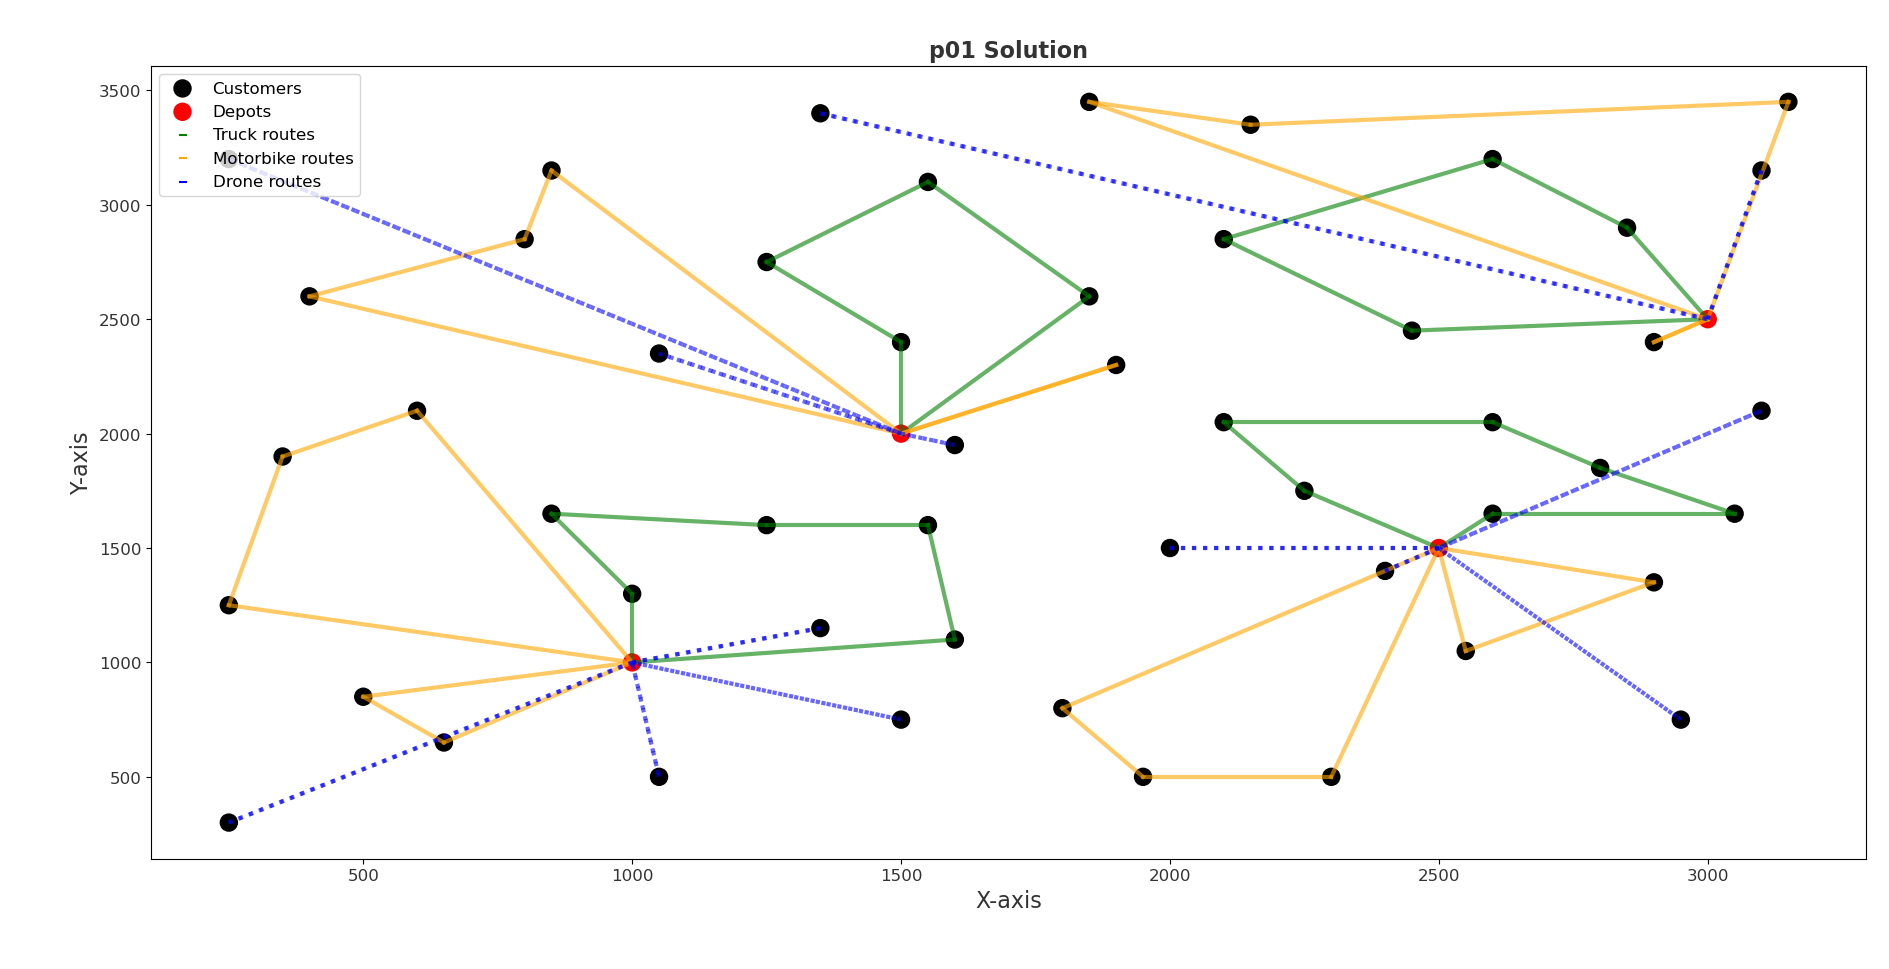
\includegraphics[width=0.9\textwidth]{p01_best_solution}
	\end{figure}
	\selectlanguage{greek}
	\section{Περιεχόμενα}
	\begin{itemize}
		\item \selectlanguage{greek}Υλοποίηση του \selectlanguage{english}mfcmTSP (2019) heuristic \selectlanguage{greek}, 
		με προσθήκη υποστήριξης πολλαπλών οχημάτων κάθε είδους σε κάθε αποθήκη, και χρήση τεχνικής \selectlanguage{english}cluster first-route second \selectlanguage{greek} για την προσαρμογή του αλγορίθμου στην εκδοχή του προβλήματος με πολλαπλές αποθήκες.\;
		\item Βελτίωση του αλγορίθμου και σύγκριση αποτελεσμάτων.\;
		\item Χρήση \selectlanguage{english}local search optimization \selectlanguage{greek}για την περαιτέρω βελτίωση αποτελεσμάτων.\;
		\item Παρουσίαση ενός υβριδικού \selectlanguage{english}metaheuristic \selectlanguage{greek}που κάνει χρήση του \selectlanguage{english}Ant Colony Optimization \selectlanguage{greek}σε συνδυασμό με το \selectlanguage{english} heuristic.\;
		\item \selectlanguage{greek}Σύγκριση των αλγορίθμων.\;
	\end{itemize}
	\selectlanguage{english}
	\newpage
	\subsection{Motivation / Use case}
	Consider a parcel delivery company operating in Greece, with depots located in two major cities: Athens and Thessaloniki. The company manages numerous last-mile delivery shops in these cities, which serve as depots in the routing problem. For instance, a customer in Thessaloniki sends a parcel to a friend in Athens by visiting a nearby shop. After the shop stops receiving parcels for the day, a truck collects the parcels and delivers them to the Thessaloniki distribution center. Parcels destined for Athens are then transported overnight to the Athens distribution center.
	Upon arrival, parcels are sorted based on their delivery areas and sent to the appropriate last-mile shops in Athens. These shops, acting as depots in our problem, dispatch vehicles (Trucks, Motorbikes, Drones) to deliver the parcels to their final destinations. \textbf{The MD-mfcmTSP addresses how these vehicles can be optimally routed to minimize delivery time, while simultaneously solving the problem of parcel allocation in each last-mile shop}.
	\par
	\begin{figure}[h!]
		\caption{Life of a parcel}
		\centering
		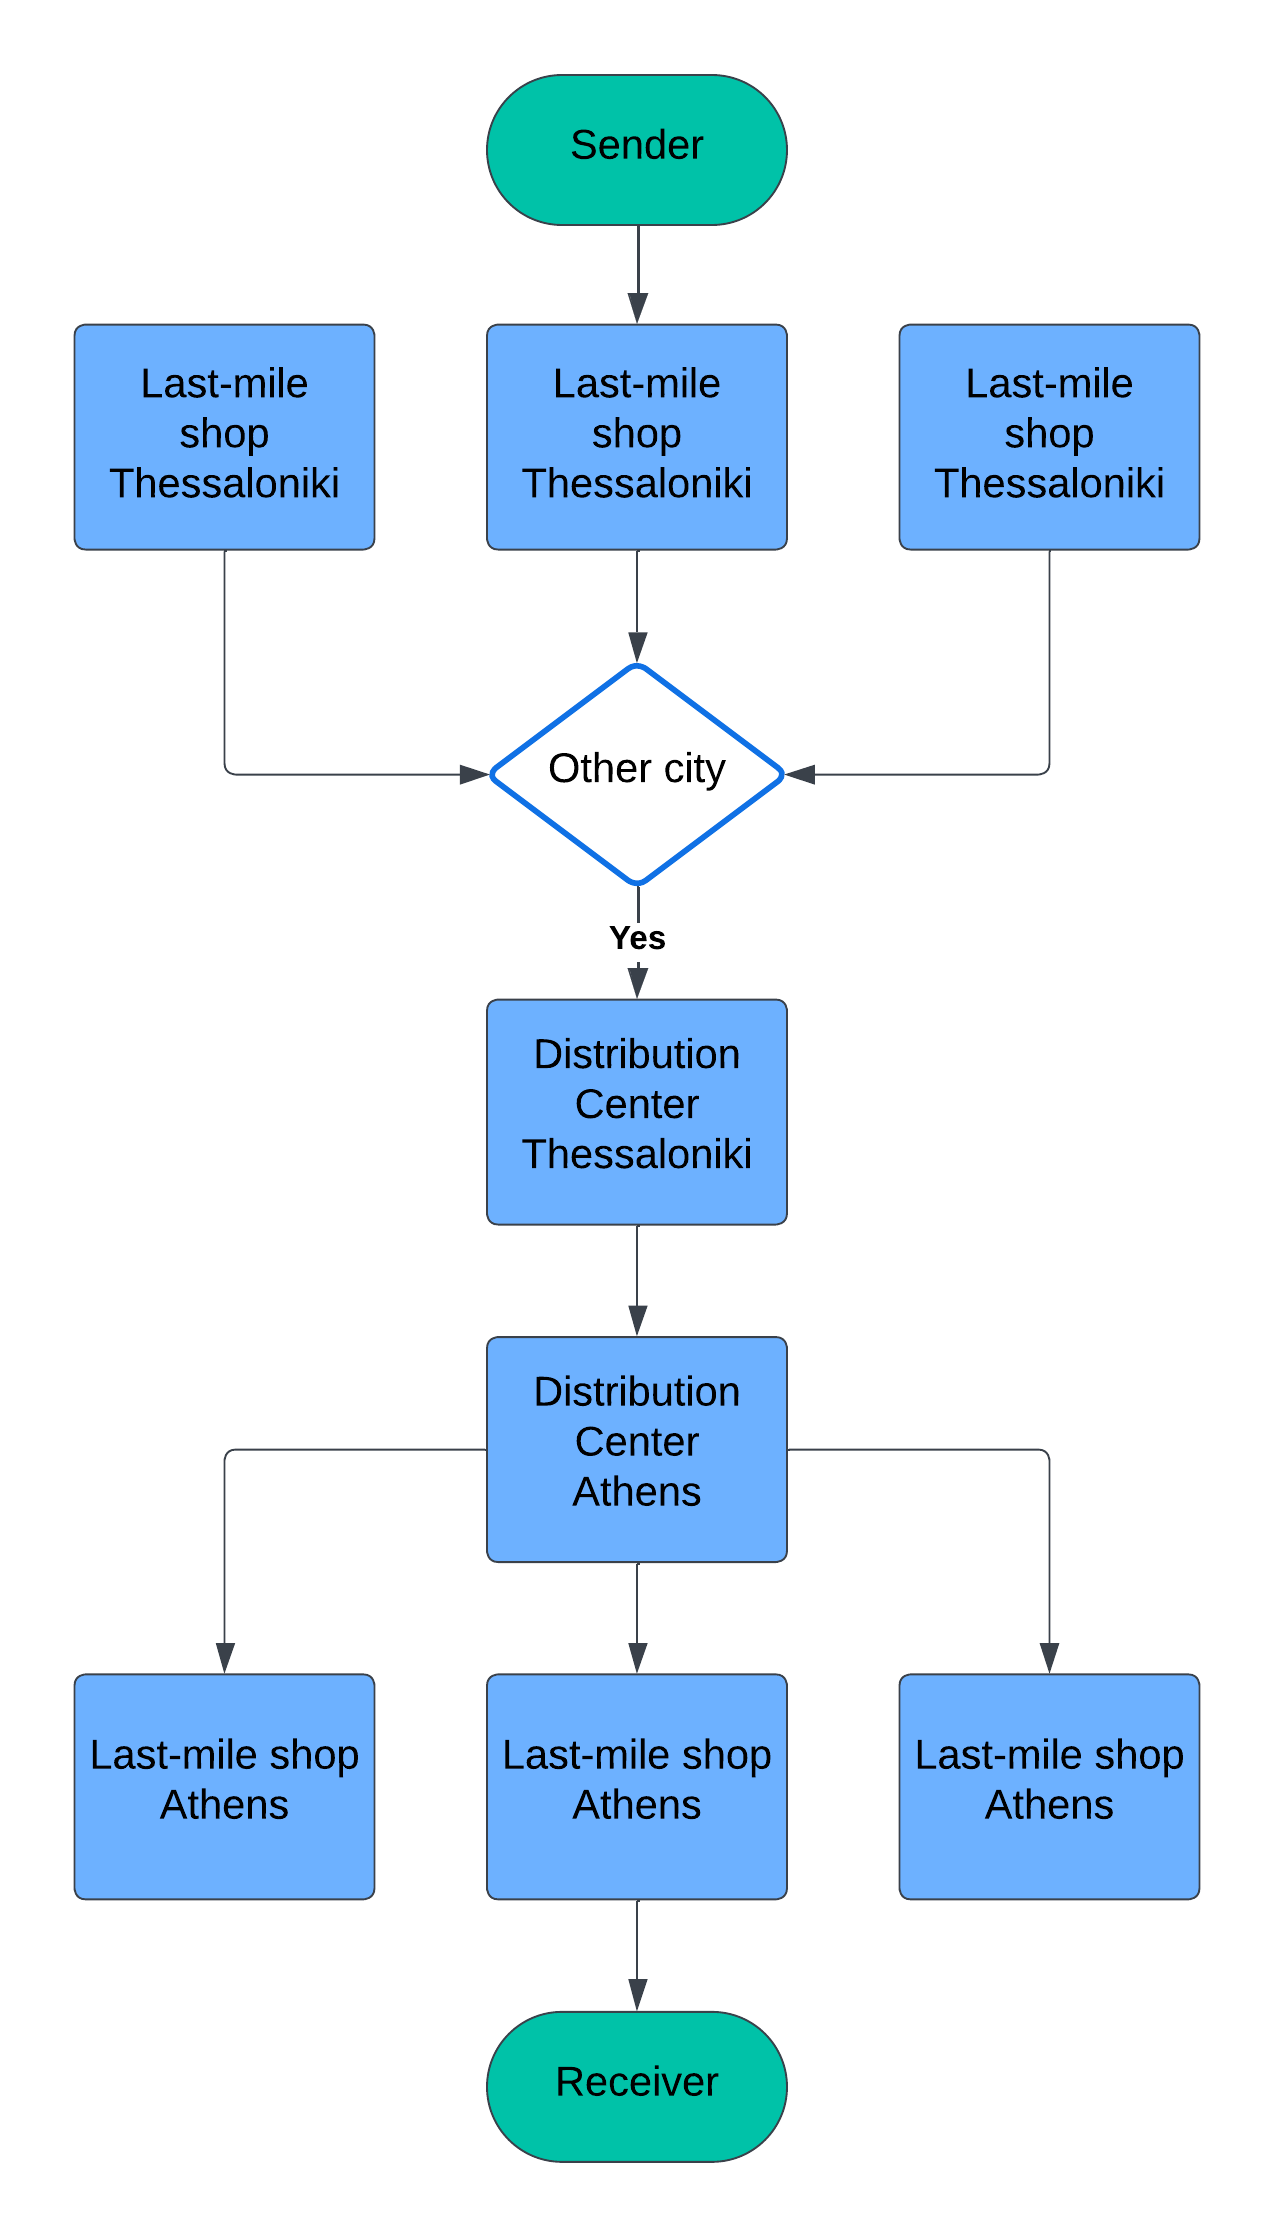
\includegraphics[width=0.40\textwidth, height=0.50\textheight]{Parcel-Life}
	\end{figure}
	\newpage
	\section{Objective}
	The objective of the MD-mfcmTSP is to minimize the total makespan in which all customers are visited/served i.e min $M_{total}$.\;
	\newline
	\newline
	\textbf{Notation}\;
	\begin{itemize}
		\item $m$ : Number of depots
		\item $D$ : Set of depots
		\item $R_T^i$ : Truck route of depot $i\in D$ \;
		\item $R_M^i$ : Motorbike route of depot $i\in D$ \;
		\item $R_D^i$ : Drone route of depot $i\in D$ \;
		\item $M_T^i$ : Time of the Truck's route(s) ($N^i_{T}=1$) or Makespan of the Trucks' route(s) ($N^i_{T}>1$) of depot $i\in D$ \;
		\item $M_M^i$ : Time of the Motorbike's route(s) ($N^i_{M}=1$) or Makespan of Motorbikes' route(s) ($N^i_{M}>1$) of depot $i\in D$ \;
		\item $M_D^i$ : Time of the Drone's route(s) ($N^i_{D}=1$) or Makespan of Drones' route(s) ($N^i_{D}>1$) of depot $i\in D$ \;
		\item $M^i_{total}=max(M_T^i,M_M^i,M_D^i)$ : Makespan of depot $i\in D$\; 
		\item $M_T$ = $max(M_T^i, M_T^{i+1}, ..., M_T^m)$ : Makespan of Trucks \;
		\item $M_M$ = $max(M_M^i, M_M^{i+1}, ..., M_M^m)$ : Makespan of Motorbikes \;
		\item $M_D$ = $max(M_D^i, M_D^{i+1}, ..., M_D^m)$ : Makespan of Drones \;
		\item $M_{total}$ = $max(M_T, M_M, M_D)$ : Total makespan \;
		\item $M_{total}$ = $max(M_{total}^i, M_{total}^{i+1}, ..., M_{total}^m)$ : Total makespan\;
	\end{itemize}
	\begin{table}[h!]
	\centering
	\caption{Example}
	\resizebox{0.3\columnwidth}{!}{%
		\begin{tabular}{@{}ccccc@{}}
			\toprule
			\textbf{Depot} & \textbf{$M_T$} & \textbf{$M_M$} & \textbf{$M_D$} & \textbf{Depot makespan} \\ 
			\midrule
			1 & 3 & 2 & 1 & 3 \\
			\midrule 
			2 & 4 & 3 & 2 & 4 \\
			\midrule 
			3 & 1 & 5 & 2 & 5 \\
			\midrule 
			4 & 2 & 8 & 1 & 8 \\
			\midrule
			\textbf{$M_{total}$} & 4 & \textbf{8} & 2 & \textbf{8} \\
			\bottomrule
		\end{tabular}%
	}
\end{table}
	\newpage
	\subsection{Makespan calculations}
	In the case where a depot is equipped with more than 1 vehicle of any type (excluding vehicles with capacity = 1 i.e drones), and two or more routes need to be assigned to them, a \textbf{job scheduling problem} arises, where the routes are the jobs that need to be assigned to machines (vehicles). Since the vehicles are identical, it's more specifically an \textbf{identical-machines scheduling problem}. Minimizing the maximum completion time (makespan) is NP-hard. Many exact and approximation algorithms are known. We use the \textbf{longest-processing-time-first (LPT)} greedy algorithm, which orders the jobs by descending order of their cost and then schedules each job in this sequence into the machine of which the current load is smallest.
	An example is given below.
	Assume 4 routes that need to be assigned to two trucks. Each route has a time cost associated with it. The route assignment needs to be done in such a way that the trucks' makespan is minimized. We first sort the routes based on their cost in a descending order. Then, starting from the route with the maximum cost, we assign it to the truck with the currently minimum makespan. This is done iteratively until all routes have been assigned to a vehicle. 
	\begin{table}[h!]
	\centering
	\caption{4 routes that need to be assigned to a depot's 2 trucks}
	\resizebox{0.12\columnwidth}{!}{%
		\begin{tabular}{@{}cc@{}}
			\toprule
			\textbf{Route} & \textbf{Cost} \\ 
			\midrule
			1 & 5 \\
			\midrule 
			2 & 6 \\
			\midrule 
			3 & 2 \\
			\midrule 
			4 & 3 \\
			\bottomrule
		\end{tabular}%
	}
\end{table}
\newline
\textbf{Procedure for the assignment of 4 routes to 2 trucks of the same depot:}
\begin{table}[h!]
	\centering
	\caption{Sort routes in descending order based on cost}
	\resizebox{0.12\columnwidth}{!}{%
		\begin{tabular}{@{}cc@{}}
			\toprule
			\textbf{Route} & \textbf{Cost} \\ 
			\midrule
			2 & 6 \\
			\midrule 
			1 & 5 \\
			\midrule 
			4 & 3 \\
			\midrule 
			3 & 2 \\
			\bottomrule
		\end{tabular}%
	}
\end{table}
\begin{table}[h!]
	\centering
	\caption{Iteratively assign routes to Trucks}
	\resizebox{0.5\columnwidth}{!}{%
		\begin{tabular}{@{}cccccc@{}}
			\toprule
			\textbf{Iteration} & \textbf{Route} & \textbf{Cost} & \textbf{Truck} & \textbf{Truck 1 ms} & \textbf{Truck 2 ms}\\ 
			\midrule
			1 & 2 & 6 & 1 & 6 & 0\\
			\midrule 
			2 & 1 & 5 & 2 & 6 & 5\\
			\midrule 
			3 & 4 & 3 & 2 & 6 & 8\\
			\midrule 
			4 & 3 & 2 & 1 & 8 & 8\\
			\midrule
			\multicolumn{6}{@{}c@{}}{Total makespan = 8 (optimal)}\\
			\bottomrule
		\end{tabular}%
	}
\end{table}
	\newpage
	\twocolumn
	
	\section{Pseudocode for the MD-mfcmTSP heuristic}
	\begin{algorithm}
		\small
		\caption{MD-mfcmTSP heuristic}
		\label{alg:MDmfcmTSP}
		\KwIn{$G_T, G_M, ..., G_D$}
		\KwOut{$M_{total}$, $Sol = \{Sol^i = \{R_T^i, R_M^i, ...,R_D^i\}, Sol^{i+1}, ..., Sol^m\}$ for each $i\in D$}
		
		Create clusters $K^i$ of customer nodes for each depot $d^i\in D$\;
		by assigning each customer to the closest possible depot\;
		\For{each $d^i\in D$}{
			
			Call $Initialization(d^i, K^i)$\;
			\While{$(M_T^i > M_M^i\parallel M_T^i > M_D^i)$ $\&\&$ $stop\neq true$}{
				$diff_M = M_T^i - M_M^i$\;
				$diff_D = M_T^i - M_D^i$\;
				\uIf{$diff_M\ge diff_D$}{
					$vt = M$\;
					$cap =$ Motorbike's capacity\;
				}\Else{
					$vt = D$\;
					$cap =$ 1\;
				}
				$M_{dep} = M_T^i$\;
				$r_{best} = \emptyset$\;
				\For{$j=1$ to $|R_T^i| - cap$}{
					$successive\_nodes = \emptyset$\;
					$load = 0$\;
					\While{$load + v_j^{demand} \leq cap$ $\&\&$ $v_j\in G_{vt}$}{
						$successive\_nodes \pluseq v_j$\;
					}
					\If{$|successive\_nodes| == cap$}{
						$r_{new} = R_T^i[0] + \{successive\_nodes\} + R_T^i[0]$\;
						${R'}_{vt}^i = R_{vt}^i + r_{new}$\;
						${M'}_{vt} = {R'}_{vt}^i$ 's makespan\;
						${R'}_T^i = R_T^i - \{successive\_nodes\}$\;
						${M'}_T = {R'}_T^i$ 's makespan\;
						$M_{new} = MAX({M'}_T, {M'}_{vt})$\;
						\If{$M_{new} < M_{dep}$}{
							$M_{dep} = M_{new}$\;
							$r_{best} = r_{new}$\;
						}
						$r_{new} = \emptyset$\;
					}
					$j\pluseq 1$\;
				}
				\uIf{$r_{best} \neq \emptyset$}{
					$R_T^i = R_T^i - \{r_{best}^{customers}\}$\;
					$M_T = R_T^i$ 's makespan\;
					$R_{vt}^i\pluseq r_{best}$\;
					$M_{vt} = R_{vt}^i$ 's makespan\;
					(+Swap)\;
					Call $local\_optimization(R_T^i, n_{max})$\;
					Call $local\_optimization(R_{vt}^i, n_{max})$\;
				}\Else{ 
					$stop = true$\;
				}
			}
			$Sol^i = \{R_T^i, R_M^i, ..., R_D^i\}$\;
		}
		$M_T = MAX(M_T^i, M_T^{i+1}, ..., M_T^m)$\;
		$M_M = MAX(M_M^i, M_M^{i+1}, ..., M_M^m)$\;
		$M_D = MAX(M_D^i, M_D^{i+1}, ..., M_D^m)$\;
		$M_{total} = MAX(M_T, M_M, ..., M_D)$\;
		Call $optimization\_full(Sol, n_{max})$
	\end{algorithm}
	
	\begin{algorithm}
		\small
		\caption{Initialization($d^i, K^i$)}
		\label{alg:initialization}
		\While{$\{K^i\}\cap \{G_T\}\neq \emptyset$}{
			$R_T^i\pluseq NearestNeighbour(\{K^i\}\cap \{G_T\})$\;
		}
		$M_T^i = R_T^i$ 's makespan\;
		$v_{free} = \{K^i\} - \{G_T\}$\;
		\uIf{$v_{free} = \emptyset$}{
			\Return{$R_T^i$}\;
		}\Else{
			\While{$v_{free}\neq \emptyset$}{
				\uIf{$M_T - M_M\geq M_T - M_D \parallel G_D = \emptyset$}{
					$R_M^i\pluseq NearestNeighbour(\{K^i\}\cap \{G_M\})$\;
					$v_{free} = v_{free} - \{R_M^i\}$\;
					$M_M^i = R_M^i$ 's makespan\;
				}\Else{
					$R_D^i\pluseq closest(\{K^i\}\cap \{G_D\})$\;
					$M_D^i = R_D^i$ 's makespan\;
				}
			}
		}
		\Return{$Sol^i$}\;
	\end{algorithm}
	
	\begin{algorithm}
		\small
		\caption{$optimization\_full(Sol, n_{max})$}
		\Do{any route improves}{
		Call $vt\_optimization(Sol, n_{max} = 2)$\;
		\For{each $vt$}{
			\For{each $i\in D$}{
				Call $local\_optimization(R_{vt}^i, n_{max}=2)$\;
			}
			Call $mutual\_depot\_optimization(R_{vt}, n_{max}=2)$\;
		}
	}
	\end{algorithm}
	
	\begin{algorithm}
		\small
		\caption{$local\_optimization(r, n_{max})$}
		\For{$n=1$ to $n_{max}$}{
			\ForEach{combination of $n$ successive nodes on the route}{
				move the node(s) to a different place on the same route\;
				evaluate the new route\;
				\uIf{this route is better than the original and all constraints are satisfied}{
					replace the original route with the new one\;
				}
				continue in point 3 unless all possible places in the route have been evaluated\;
			}
		}
		\Return{$r$}\;
	\end{algorithm}
	
	\begin{algorithm}
		\small
		\caption{$mutual\_depot\_optimization(R_{vt}, n_{max})$}
		\For{$n = 1$ to $n_{max}$}{
			\ForEach{possible pair of depots $c1$ and $c2$}{
				\ForEach{combination of $n$ successive nodes in the route of c1}{
					remove the nodes from the route of c1 and insert them into c2\;
					evaluate the newly-created routes\;
					\uIf{$MAX(|{R'}_{vt}^{c1}|, |{R'}_{vt}^{c2}|) < MAX(|{R}_{vt}^{c1}|, |{R}_{vt}^{c2}|)$ and all constraints are satisfied}{
						replace the original routes with the new ones\;
					}
					continue in point 4 unless all possible places in c2 have been evaluated\;
				}
			}
		}
		\Return{$R_{VT}$}\;
	\end{algorithm}
	
	\begin{algorithm}
		\small
		\caption{$vt\_optimization(Sol, n_{max})$}
		\For{$n = 1$ to $n_{max}$}{
			\ForEach{depot $i\in D$}{
				\ForEach{possible pair of vehicle types $t1,t2\in VT$}{
					\ForEach{combination of $n$ successive nodes in $R_{t1}^i$}{
						remove the nodes from $R_{t1}^i$ and insert them in $R_{t2}^i$\;
						\uIf{$MAX(|{R'}_{t1}^i|, |{R'}_{t2}^i|) < MAX(|{R}_{t1}^i|, |{R}_{t2}^i|)$ and all constraints are satisfied}{
							replace the original routes with the new ones\;
						}
						continue in point 5 unless all possible places in $R_{t2}^i$ have been evaluated\;
					}
				}
			}
		}
		\Return{$Sol$}\;
	\end{algorithm}
	\clearpage
	\section{Solving the MD-mfcmTSP}
	In this section, we introduce the two algorithmic approaches to address the MD-mfcmTSP. The first approach which is used to tackle the problem comprises of a clustering phase, which transforms the multi-depot problem into multiple single-depot mfcmTSP problems, and a routing phase which calls the mfcmTSP heuristic for each depot. The second approach leverages a hybrid metaheuristic, combining Ant Colony Optimization (ACO) with the mfcmTSP heuristic.
	\subsection{MD-mfcmTSP heuristic}
	To manage the complexity of multi-depot routing problems, a widely used approach is their transformation to multiple single-depot routing problems. Although a naive approach, it provides feasible solutions of which the results are used as a baseline for comparison with other solution methods.
	\par 
	For this purpose, we use a straightforward constrained proximity clustering to assign customers to depots, and then run the mfcmTSP heuristic for each depot. Each customer is assigned to the closest \textit{possible} depot, creating clusters where each depot serves the customers nearest to it. Specifically, vehicle availability at each depot may limit the customers that are assigned to its cluster. The reason is that the initialization phase of the heuristic, which is based on these clusters, must form routes that visit every node $c_i\in C$. Therefore, while the assignment is based on proximity, we must adjust the clustering to account for these constraints. This means that some customers may need to be assigned to a more distant depot if the nearest depot lacks the vehicle that can serve them. For example, a customer only accessible by motorbike will be assigned to a more distant depot when the closest to them doesn't have a motorbike available in its fleet.
	\begin{figure*}[h]
		\caption[width=\textwidth]{Initialization example}
		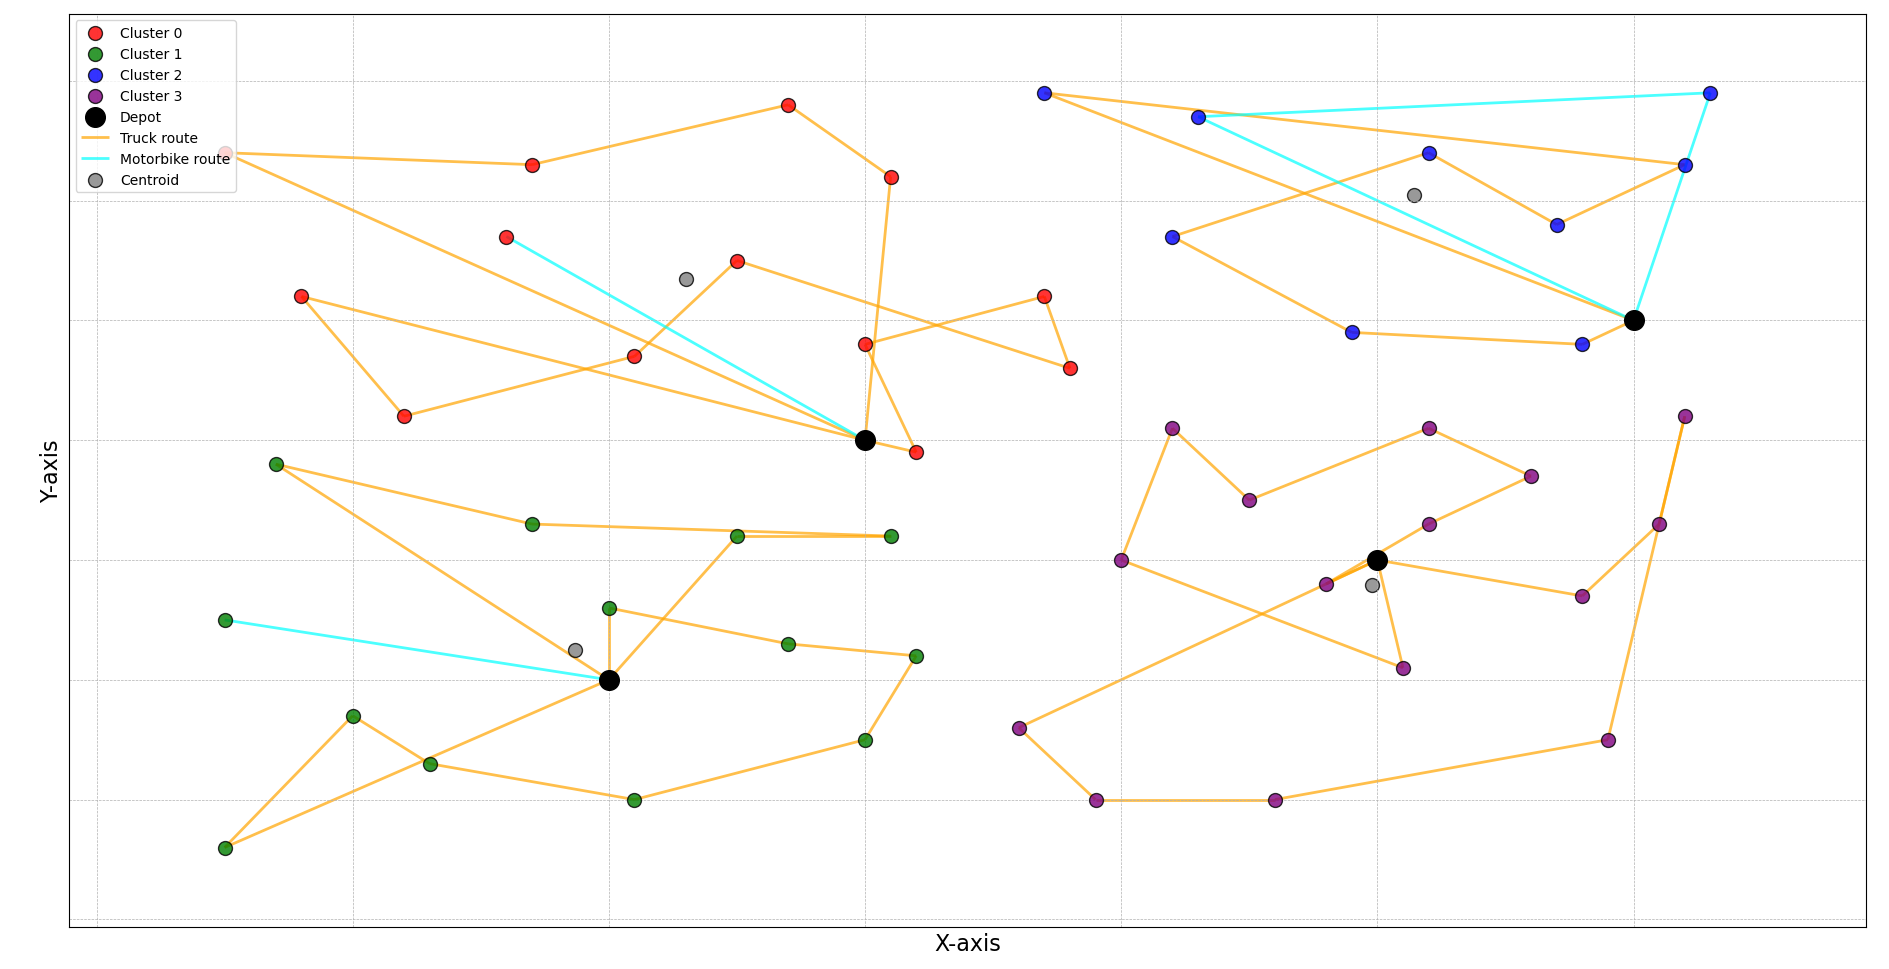
\includegraphics[width=\textwidth]{Initialization_example_p01}
		\centering
	\end{figure*}
	\begin{figure*}[h]
		\caption[width=\textwidth]{Initialization example}
		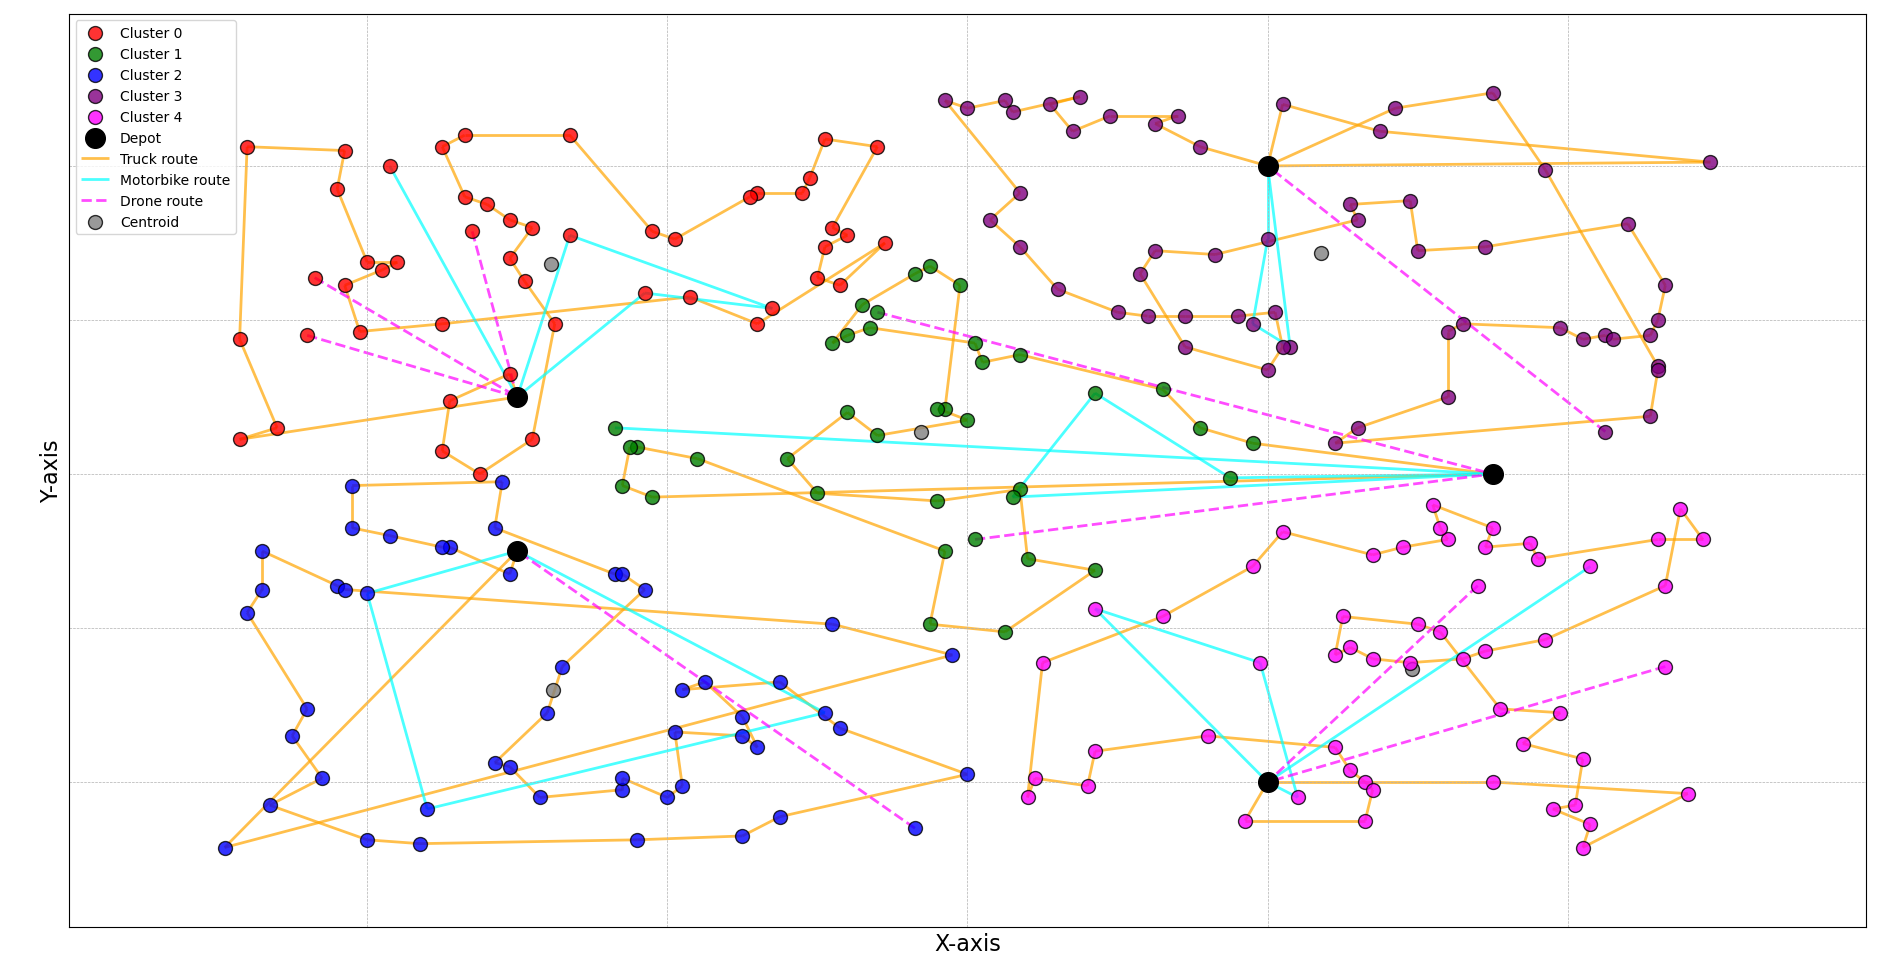
\includegraphics[width=\textwidth]{Initialization_example_p11}
		\centering
	\end{figure*}
	\begin{figure*}[h]
		\caption[width=\textwidth]{Solution after mutual depot optimization}
		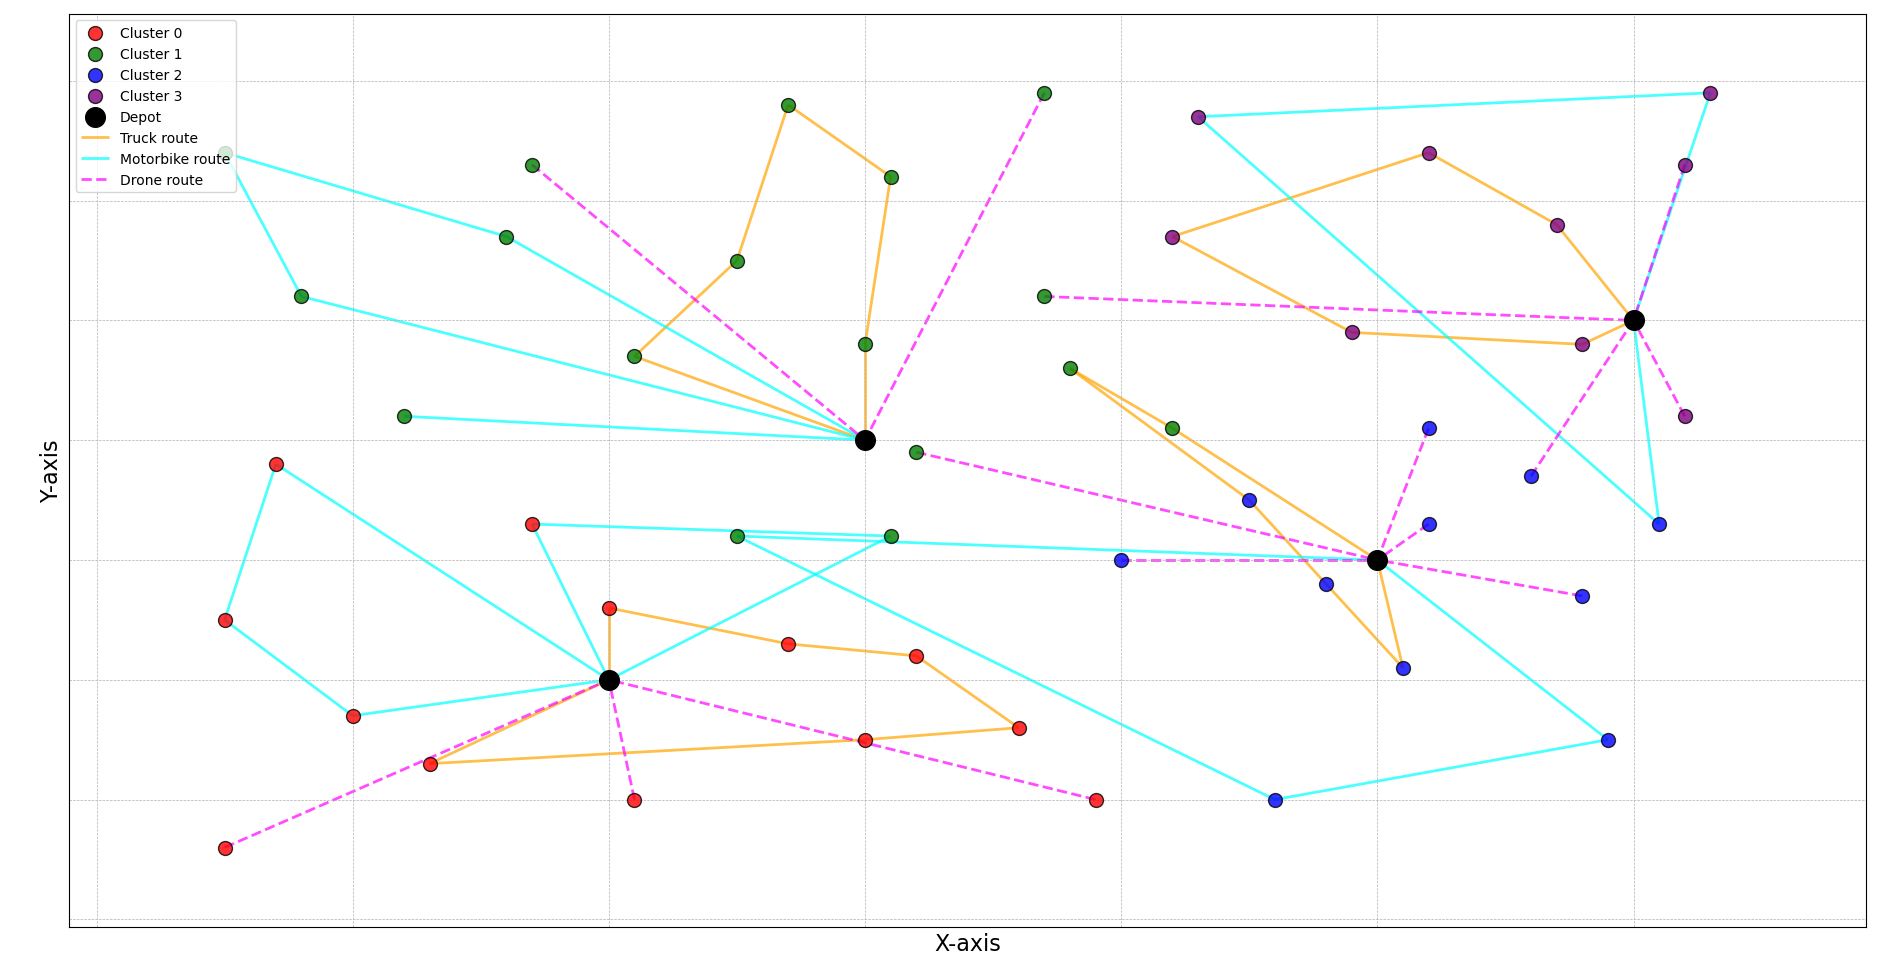
\includegraphics[width=\textwidth]{solution_p01_prox}
		\centering
	\end{figure*}
	\clearpage
	\subsection{Hybrid Ant Colony Optimization}
	For the second approach to solve the MD-mfcmTSP we introduce a novel hybrid metaheuristic based on the principles of Ant Colony Optimization combined with the mfcmTSP heuristic. Specifically, we employ a modified version of the Adaptive Ant Colony Optimization with Node Clustering (AACONC) (Stodola et al. 2022) which was developed for the Multi-Depot Vehicle Routing Problem and showed promising results. From now on, we refer to this algorithm as the H-AACONC.
	\par 
	\subsubsection{H-AACONC Algorithm}
	The Ant Colony part of the algorithm disregards accessibility constraints and assumes that all customers must be served by trucks such as to minimize the total time (makespan). As such, the pheromone matrix, node clustering and the AntSolution function remain the same as in AACONC and are used to create an initial trucks-only solution which is stored in $Rt$. Then, with  frequency $n_{freq}$, which is one of the AACONC control parameters, the single and mutual colony local optimization procedures may be called. In the resulting solution $Rt$, customers that are not accessible by trucks are then offloaded to the motorbike(s) of the same depot if possible, else to the closest depot with atleast one motorbike in its fleet. The resulting routes are inserted into $R_{best}$ and the MD-mfcmTSP heuristic is called, while skipping the clustering and initialization phase.
	\subsubsection{Pheromone matrix update}
	One key distinction between the AACONC and the H-AACONC is the pheromone matrix update procedure.
	The pheromone matrix update procedure uses the same logic as the AACONC. The Simulated Annealing principle in combination with the Metropolis criterion probabilistically decide which solution will be used for the update. Although in the H-AACONC, while solutions $R$ and $R_{best}$ are used to make this decision, it is then truck solutions $Rt$ and $Rt_{best}$ respectively that are used to update the pheromone matrix.
	\begin{equation}
		p(R^{best}) = 1 - p(R) = 
		\begin{cases}
			e^{-\frac{(|R^{best}| - |R|)/|R|}{T_{update}}} & \text{for } |R^{best}| > |R|, \\
			1 & \text{otherwise}
		\end{cases}
	\label{eq:SA}
	\end{equation}
	\begin{equation}
	 	T_{\text{update}}(iter + 1) = \alpha_{\text{update}} \cdot T_{\text{update}}(iter)
	\label{eq:Tupdate}
	\end{equation}
	The solution for updating the pheromone matrix $R^{update}$ is selected based on the calculated probabilities:
	$R^{update} = R^{best}$ and $Rt^{update} = Rt^{best}$with $p(R^{best})$ or $R^{update} = R$ and $Rt^{update} = Rt$ with $p(R) = 1 - p(R^{best})$.The update itself is then conducted using (\ref{eq:phUpdate}); the pheromone trails lying on the routes are increased in proportion to the pheromone
	updating coefficient $\delta$ and the quality of the updating route (a ratio of $R$ to $R^{update}$).
	\begin{equation}
			\tau_{ij}^k = \tau_{ij}^k + \chi_{ij}\cdot \delta \cdot \frac{|R|}{|R^{update}|} \text{ for all } v_i,v_j \in V \text{ and } d_k\in D
			\label{eq:phUpdate}
	\end{equation}
	\begin{equation}
		\chi_{ij} = 
		\begin{cases}
			1 & \text{if there is an edge between }v_i \text{ and }v_j \text{ in }Rt^{update},\\
			0 & \text{otherwise}
		\end{cases}
	\end{equation}
	\begin{algorithm}
	\small
	\caption{Hybrid AACONC}
	\label{alg:H-AACONC}
	\KwIn{$G_T, G_M, G_D, k_T, k_M$}
	\KwOut{$M_{total}$, $Sol = \{Sol^i = \{R_T^i, R_M^i, R_D^i\}, Sol^{i+1}, ..., Sol^m$ for each $i\in D\}$}
	$iter$ = 0\;
	Initialize pheromone matrices $\tau$\;
	\ForEach{$v_i\in V$}{
		$K^{(v_i)}$ = Call CreateClusters\;
	}
	$Rt=\infty,R=\infty$\;
	\While{NOT TERMINATED}{
		$Rt_{best}=\infty,R_{best}=\infty$\;
		\ParallelFor{$\alpha=1$ to $n_{ants}$}{
			$R_a$ = \textbf{Call AntSolution} \;
			//which  construct routes using Trucks for every $c\in C$\;
			\KwCritical{
				\If{$|R_a|<|Rt_{best}|$}{
				$Rt_{best}=R_a$\;
				}
			}
		}	
		\If{$iter$ mod $n_{freq}$=0}{
			$Rt_{best}$ = Call $local\_optimization$\;
			$Rt_{best}$ = Call $mutual\_depot\_optimization$\;
		}
		Assign customers in $Rt_{best}$ which do not belong to $G_T$ to $R_{best}^M,R_{best}^D$\;
		$R_{best}^T=Rt_{best}-\{R_{best}^M,R_{best}^D\}$\;
		$R_{best}$ = Call MD-mfcmTSP heuristic\;
		\If{$|R_{best}| < |R|$}{
			$R=R_{best}$\;
			$Rt=Rt_{best}$\;
		}
		Update pheromones\;
		Evaporate pheromones\;
		$iter\pluseq 1$\;
	}
\end{algorithm}\;
	\onecolumn
	\section{Instances}
	% Please add the following required packages to your document preamble:
% \usepackage{booktabs}
% \usepackage{graphicx}
\begin{table}[h]
	\centering
	\begin{minipage}{0.7\columnwidth}
	\centering
	\caption{MD-mfcmTSP Instances}
	\resizebox{\columnwidth}{!}{%
		\begin{tabular}{@{}ccccccc@{}}
			\toprule
			\textbf{Instance} & \textbf{Customers} & \textbf{Depots} & \textbf{Dimensions} & \textbf{$C^{Truck}$} & \textbf{$C^{UAV}$} \\
			\midrule
			1 & 50 & 4 & 3150m x 3450m & 46 & 42 \\
			\midrule
			2 & 50 & 4 & 3150m x 3450m & 46 & 40 \\
			\midrule
			3 & 75 & 5 & 3500m x 3800m & 64 & 62\\
			\midrule
			4 & 100 & 2 & 3350m x 3850m & 88 & 87 \\
			\midrule
			5 & 100 & 2 & 3350m x 3850m & 91 & 82 \\
			\midrule
			6 & 100 & 3 & 3350m x 3850m & 91 & 85 \\
			\midrule
			7 & 100 & 4 & 3350m x 3850m & 97 & 83 \\
			\midrule
			8 & 249 & 2 & 9900m x 9800m & 219 & 215 \\
			\midrule
			9 & 249 & 3 & 9900m x 9800m & 224 & 212 \\
			\midrule
			10 & 249 & 4 & 9900m x 9800m & 223 & 221 \\
			\midrule
			11 & 249 & 5 & 10500m x 5000m & 222 & 208 \\
			\midrule
			12 & 500 & 4 & 7500m x 7500m & 461 & 425 \\
			\midrule
			13 & 500 & 4 & 7500m x 7500m & 448 & 436 \\
			\midrule
			14 & 500 & 5 & 7500m x 7500m & 458 & 413 \\
			\midrule
			15 & 1000 & 4 & 10000m x 10000m & 903 & 855 \\
			\midrule
			16 & 1000 & 6 & 10000m x 10000m & 887 & 842 \\
			\bottomrule
		\end{tabular}%
	}
	\label{tab:instances_table}
\end{minipage}
\end{table}\;
	% Please add the following required packages to your document preamble:
% \usepackage{booktabs}
% \usepackage{graphicx}
\begin{table*}[h]
	\begin{minipage}{0.6\columnwidth}
		\centering
		\caption{MD-mfcmTSP new generated Instances}
		\resizebox{\textwidth}{!}{%
			\begin{tabular}{@{}cccccc@{}}
				\toprule
				\textbf{Instance} & \textbf{Customers} & \textbf{Depots} & \textbf{Dimensions} & \textbf{Truck capacity}& \textbf{Layout} \\
				\midrule
				x01 & 500 & 4 & 7500m x 7500m & 100 & Random \\
				\midrule
				x02 & 500 & 4 & 7500m x 7500m & 100 & Random \\
				\midrule
				x03 & 500 & 5 & 7500m x 7500m & 100 & Random \\
				\midrule
				x04 & 1000 & 4 & 10000m x 10000m & 100 & Random \\
				\midrule
				x05 & 1000 & 6 & 10000m x 10000m & 100 & Random \\
				\bottomrule
			\end{tabular}%
		}
	\end{minipage}
\end{table*}\;
	\clearpage
	\section{Results}
	\subsection{New heuristic vs original heuristic}
	\textbf{mfcmTSP heuristic (original) : } Finds and swaps the minimum cost route in each iteration \\ \;
	\\
	\par
	\textbf{MD-mfcmTSP heuristic (v1) : } Finds and swaps the route which minimizes the depot's makespan in each iteration \\ \;
	\par 
	Results show that the new (v1) heuristic performs better than the original.
		
	\begin{table}[h]
		\centering
		\caption{Comparison of the two algorithms ($S_T = 15, S_M = 25, S_D = 30$)}
		\resizebox{\textwidth}{!}{ % Resize the table to fit the page width
			\begin{tabular}{ccccccccccccccc}
				\toprule
				\textbf{Instance} & \textbf{Best} & \multicolumn{6}{c}{\textbf{new (v1)}} & \multicolumn{6}{c}{\textbf{original}} \\
				\cmidrule(lr){3-8} \cmidrule(lr){9-14}
				& & \textbf{+Swap} & \textbf{gap} & \textbf{Standard} & \textbf{gap} & \textbf{No Local} & \textbf{gap} & \textbf{+Swap} & \textbf{gap} & \textbf{Standard} & \textbf{gap} & \textbf{No Local} & \textbf{gap} \\
				\midrule
				p01 & 215.15 & 217.42 & 1.06 & \textbf{215.15} & 0.00 & 334.04 & 55.26 & 243.72 & 13.28 & 232.34 & 7.99 & 356.47 & 65.68 \\
				p02 & 218.40 & 219.20 & 0.37 & \textbf{218.40} & 0.00 & 308.83 & 41.41 & 243.72 & 11.59 & 221.55 & 1.44 & 372.28 & 70.46 \\
				p03 & 202.43 & 214.84 & 6.13 & \textbf{202.43} & 0.00 & 253.13 & 25.07 & 277.50 & 37.08 & 218.73 & 8.05 & 347.94 & 71.88 \\
				p04 & 668.81 & \textbf{668.81} & 0.00 & 711.80 & 6.43 & 779.34 & 16.53 & 711.00 & 6.31 & 740.45 & 10.71 & 924.31 & 38.20 \\
				p05 & 630.78 & \textbf{630.78} & 0.00 & 655.40 & 3.90 & 726.62 & 15.19 & 713.20 & 13.07 & 713.39 & 13.08 & 874.80 & 38.69 \\
				p06 & 431.32 & 435.42 & 0.95 & \textbf{431.32} & 0.00 & 650.37 & 50.77 & 481.20 & 11.56 & 471.61 & 9.34 & 751.05 & 74.13 \\
				p07 & 309.48 & \textbf{309.48} & 0.00 & 349.19 & 12.83 & 350.77 & 13.34 & 322.29 & 4.15 & 359.18 & 16.06 & 589.22 & 90.39 \\
				p08 & 3079.58 & 3333.93 & 8.26 & \textbf{3079.58} & 0.00 & 3321.63 & 7.86 & 3448.84 & 11.99 & 3380.67 & 9.78 & 4009.10 & 30.18 \\
				p09 & 1917.82 & \textbf{1917.82} & 0.00 & 2102.98 & 9.68 & 2429.24 & 26.67 & 2201.39 & 14.79 & 2157.10 & 12.48 & 2732.05 & 42.46 \\
				p10 & 1493.13 & \textbf{1493.13} & 0.00 & 1525.37 & 2.16 & 1864.23 & 24.85 & 1630.94 & 9.23 & 1614.27 & 8.11 & 2437.73 & 63.26 \\
				p11 & 1096.74 & 1145.75 & 4.47 & 1101.33 & 0.42 & 1239.36 & 13.00 & 1213.34 & 10.45 & \textbf{1096.74} & 0.00 & 1583.09 & 44.35 \\
				\midrule
				\textbf{Average} & 933.05 & 962.41 & \textbf{1.93\%} & 962.99 & 3.21\% & 1114.32 & 26.35\% & 1044.08 & 13.04\% & 1018.73 & 8.82\% & 1361.64 & 57.24\% \\
				\bottomrule
				\toprule
				x01 & 1454.47 & 1550.64 & 6.61\% & \textbf{1454.47} & 0.00\% & 1886.98 & 29.74\% & 1542.40 & 6.05\% & 1651.89 & 13.57\% & 2411.57 & 65.80\% \\
				x02 & 1514.61 & \textbf{1514.61} & 0.00\% & 1525.87 & 0.74\% & 1705.48 & 12.60\% & 1644.94 & 8.60\% & 1705.10 & 12.58\% & 2099.51 & 38.62\% \\
				x03 & 1306.20 & 1313.16 & 0.53\% & 1352.27 & 3.53\% & 1556.10 & 19.13\% & \textbf{1306.20} & 0.00\% & 1338.43 & 2.47\% & 1985.68 & 52.02\% \\
				x04 & 3031.00 & \textbf{3031.00} & 0.00\% & 3128.87 & 3.23\% & 3436.31 & 13.37\% & 3176.20 & 4.79\% & 3199.83 & 5.57\% & 3967.73 & 30.90\% \\
				x05 & 2046.21 & \textbf{2046.21} & 0.00\% & 2099.98 & 2.63\% & 2421.32 & 18.33\% & 2292.28 & 12.03\% & 2228.69 & 8.92\% & 3061.06 & 49.60\% \\
				\midrule
				\textbf{Average} & 1870.50 & 1891.12 & \textbf{1.43\%} & 1912.29 & 2.03\% & 2201.24 & 18.63\% & 1992.40 & 6.29\% & 2024.79 & 8.62\% & 2705.11 & 47.39\% \\
				\bottomrule
			\end{tabular}
		}

		\label{tab:comparison}
	\end{table}

\;
	\begin{table}[h]
	\centering
	\caption{Comparison of the two algorithms ($S_T = 15, S_M = 20, S_D = 30$)}
	\resizebox{\textwidth}{!}{ % Resize the table to fit the page width
		\begin{tabular}{ccccccccccccccc}
			\toprule
			\textbf{Instance id} & \textbf{Best} & \multicolumn{6}{c}{\textbf{new (v1)}} & \multicolumn{6}{c}{\textbf{original}} \\
			\cmidrule(lr){3-8} \cmidrule(lr){9-14}
			& & \textbf{+Swap} & \textbf{gap} & \textbf{Standard} & \textbf{gap} & \textbf{No Local} & \textbf{gap} & \textbf{+Swap} & \textbf{gap} & \textbf{Standard} & \textbf{gap} & \textbf{No Local} & \textbf{gap} \\
			\midrule
			p01 & 221.54 & 265.62 & 19.90\% & \textbf{221.54} & 0.00\% & 361.73 & 63.28\% & 231.04 & 4.29\% & 258.24 & 16.57\% & 410.50 & 85.29\% \\
			p02 & 224.38 & \textbf{224.38} & 0.00\% & 230.97 & 2.94\% & 314.64 & 40.23\% & 246.38 & 9.80\% & 259.42 & 15.62\% & 382.31 & 70.39\% \\
			p03 & 231.85 & 232.55 & 0.30\% & \textbf{231.85} & 0.00\% & 275.80 & 18.96\% & 277.50 & 19.69\% & 247.39 & 6.70\% & 349.68 & 50.82\% \\
			p04 & 743.39 & 771.46 & 3.78\% & \textbf{743.39} & 0.00\% & 833.11 & 12.07\% & 769.70 & 3.54\% & 768.52 & 3.38\% & 995.79 & 33.95\% \\
			p05 & 699.49 & 701.25 & 0.25\% & \textbf{699.49} & 0.00\% & 785.30 & 12.27\% & 737.73 & 5.47\% & 733.75 & 4.90\% & 927.64 & 32.62\% \\
			p06 & 473.32 & \textbf{473.32} & 0.00\% & 523.44 & 10.59\% & 715.92 & 51.25\% & 545.35 & 15.22\% & 493.64 & 4.29\% & 808.94 & 70.91\% \\
			p07 & 339.27 & 367.53 & 8.33\% & \textbf{339.27} & 0.00\% & 417.10 & 22.94\% & 352.11 & 3.78\% & 440.15 & 29.73\% & 469.11 & 38.27\% \\
			p08 & 3330.48 & 3476.45 & 4.38\% & \textbf{3330.48} & 0.00\% & 3521.95 & 5.75\% & 3586.21 & 7.68\% & 3646.71 & 9.50\% & 4312.54 & 29.49\% \\
			p09 & 2064.72 & \textbf{2064.72} & 0.00\% & 2408.35 & 16.64\% & 2583.64 & 25.13\% & 2206.32 & 6.86\% & 2436.95 & 18.03\% & 2935.01 & 42.15\% \\
			p10 & 1601.68 & 1605.77 & 0.26\% & 1655.83 & 3.38\% & 1888.36 & 17.90\% & 1625.21 & 1.47\% & \textbf{1601.68} & 0.00\% & 2437.73 & 52.20\% \\
			p11 & 1140.61 & 1195.53 & 4.81\% & \textbf{1140.61} & 0.00\% & 1345.70 & 17.98\% & 1274.27 & 11.72\% & 1274.53 & 11.74\% & 1590.39 & 39.43\% \\
			\midrule
			\textbf{Average} & 1006.43 & 1034.42 & 3.82\% & 1047.75 & \textbf{3.05\%} & 1185.75 & 26.16\% & 1077.44 & 8.14\% & 1105.54 & 10.95\% & 1419.97 & 49.59\% \\
			\bottomrule
			\toprule
			 x01 & 1578.55 & 1597.25 & 1.18\% & \textbf{1578.55} & 0.00\% & 1976.45 & 25.21\% & 1669.33 & 5.75\% & 1716.93 & 8.77\% & 2631.68 & 66.72\% \\
			x02 & 1655.28 & \textbf{1655.28} & 0.00\% & 1673.69 & 1.11\% & 1792.14 & 8.27\% & 1726.75 & 4.32\% & 1798.78 & 8.67\% & 2346.33 & 41.75\% \\
			x03 & 1361.22 & 1406.07 & 3.29\% & \textbf{1361.22} & 0.00\% & 1690.65 & 24.20\% & 1485.35 & 9.12\% & 1459.32 & 7.21\% & 2043.82 & 50.15\% \\
			x04 & 3226.24 & 3238.88 & 0.39\% & \textbf{3226.24} & 0.00\% & 3615.71 & 12.07\% & 3325.25 & 3.07\% & 3390.14 & 5.08\% & 4073.03 & 26.25\% \\
			x05 & 2201.89 & \textbf{2201.89} & 0.00\% & 2262.24 & 2.74\% & 2587.20 & 17.50\% & 2342.16 & 6.37\% & 2397.81 & 8.90\% & 3063.97 & 39.15\% \\
			\midrule
			\textbf{Average} & 2004.64 & 2019.87 & 0.97\% & 2020.39 & \textbf{0.77}\% & 2332.43 & 17.45\% & 2109.77 & 5.73\% & 2152.60 & 7.72\% & 2831.77 & 44.80\% \\
			\bottomrule
		\end{tabular}
	}
	\label{tab:comparison_new}
\end{table}
\;
	%
	\begin{table}[h]
		\centering
		\caption{Comparison of the two algorithms (k-means)}
		\resizebox{\textwidth}{!}{ % Resize the table to fit the page width
			\begin{tabular}{ccccccccccccccc}
				\toprule
				\textbf{Instance} & \textbf{Best} & \multicolumn{6}{c}{\textbf{new (v1)}} & \multicolumn{6}{c}{\textbf{original}} \\
				\cmidrule(lr){3-8} \cmidrule(lr){9-14}
				& & \textbf{+Swap} & \textbf{gap} & \textbf{Standard} & \textbf{gap} & \textbf{No Local} & \textbf{gap} & \textbf{+Swap} & \textbf{gap} & \textbf{Standard} & \textbf{gap} & \textbf{No Local} & \textbf{gap} \\
				\midrule
				p01 & \textbf{191.03} & \textbf{191.03} & 0.00 & 202.96 & 6.25 & 225.72 & 18.16 & 219.20 & 14.75 & 211.59 & 10.76 & 255.43 & 33.71 \\
				p02 & \textbf{187.17} & 188.60 & 0.76 & \textbf{187.17} & 0.00 & 209.39 & 11.87 & 200.66 & 7.21 & 231.04 & 23.44 & 276.42 & 47.68 \\
				p03 & \textbf{185.82} & \textbf{185.82} & 0.00 & 188.63 & 1.51 & 200.64 & 7.98 & 198.56 & 6.86 & 193.44 & 4.10 & 264.94 & 42.58 \\
				p04 & \textbf{692.11} & 694.96 & 0.41 & 700.95 & 1.28 & 807.71 & 16.70 & \textbf{692.11} & 0.00 & 701.98 & 1.43 & 976.88 & 41.15 \\
				p05 & \textbf{624.33} & \textbf{624.33} & 0.00 & 629.61 & 0.84 & 697.03 & 11.63 & 692.40 & 10.90 & 672.66 & 7.74 & 901.03 & 44.35 \\
				p06 & \textbf{416.25} & \textbf{416.25} & 0.00 & 417.09 & 0.20 & 492.31 & 18.27 & 448.19 & 7.67 & 429.34 & 3.14 & 563.15 & 35.29 \\
				p07 & \textbf{313.57} & 314.41 & 0.27 & \textbf{313.57} & 0.00 & 378.90 & 20.83 & 329.90 & 5.21 & 326.80 & 4.22 & 482.11 & 53.75 \\
				p08 & \textbf{3051.63} & 3186.02 & 4.40 & \textbf{3051.63} & 0.00 & 3288.45 & 7.76 & 3144.43 & 3.04 & 3136.46 & 2.78 & 3853.50 & 26.28 \\
				p09 & \textbf{1932.21} & 1964.49 & 1.67 & \textbf{1932.21} & 0.00 & 2118.71 & 9.65 & 1949.26 & 0.88 & 1939.12 & 0.36 & 2566.00 & 32.80 \\
				p10 & \textbf{1463.63} & 1500.38 & 2.51 & \textbf{1463.63} & 0.00 & 1747.09 & 19.37 & 1523.75 & 4.11 & 1470.63 & 0.48 & 2089.33 & 42.75 \\
				p11 & \textbf{1031.09} & \textbf{1031.09} & 0.00 & 1060.37 & 2.84 & 1202.79 & 16.65 & 1105.26 & 7.19 & 1121.23 & 8.74 & 1445.91 & 40.23 \\
				\midrule
				\textbf{Average} & 917.16 & 936.13 & \textbf{0.91\%} & 922.52 & 1.17\% & 1033.52 & 14.44\% & 954.88 & 6.16\% & 948.57 & 6.10\% & 1243.15 & 40.04\% \\
				\bottomrule 
				\toprule
				x01 & \textbf{1507.89} & 1508.25 & 0.02 & \textbf{1507.89} & 0.00 & 1660.20 & 10.10 & 1565.29 & 3.81 & 1624.77 & 7.75 & 2029.75 & 34.61 \\
				x02 & \textbf{1548.49} & 1606.32 & 3.73 & \textbf{1548.49} & 0.00 & 1700.61 & 9.82 & 1637.58 & 5.75 & 1626.66 & 5.05 & 2091.24 & 35.05 \\
			
				x03 & \textbf{1265.68} & 1278.74 & 1.05 & \textbf{1265.68} & 0.00 & 1413.88 & 11.71 & 1288.77 & 1.82 & 1317.12 & 4.06 & 1735.64 & 37.13 \\
			
				x04 & \textbf{3240.55} & \textbf{3240.55} & 0.00 & 3257.37 & 0.52 & 3671.26 & 13.29 & 3310.12 & 2.15 & 3380.66 & 4.32 & 4386.27 & 35.36 \\
				
				x05 & \textbf{2127.93} & \textbf{2127.93} & 0.00 & 2159.94 & 1.50 & 2410.38 & 13.27 & 2169.78 & 1.97 & 2172.75 & 2.11 & 2662.10 & 25.10 \\
				\midrule
				\textbf{Average} & 1938.11 & 1952.40 & 0.96\% & 1947.87 & \textbf{0.40\%} & 2171.27 & 11.64\% & 1994.31 & 3.10\% & 2024.39 & 4.66\% & 2581.00 & 33.45\% \\
				\bottomrule 
			\end{tabular}
		}
	
		\label{tab:comparisonkmeans}
	\end{table}\;
	

	
	
	\clearpage
	\section{MD-mfcmTSP Results Analysis}
	\subsection{Local optimization impact on the heuristic}
	\subsubsection{Proximity clustering}
	% Please add the following required packages to your document preamble:
% \usepackage{booktabs}
% \usepackage{graphicx}
\begin{table*}[!ht]
	\centering
	\caption{Local optimization impact on heuristic using proximity clustering}
	\resizebox{\textwidth}{!}{%
		\begin{tabular}{@{}cccccccccc@{}}
			\toprule
			\textbf{Instance} & \textbf{Best} & \textbf{Full Local Opt} & \textbf{gap(\%)} & \textbf{No Local Opt} & \textbf{gap(\%)} & \textbf{Final Only} & \textbf{gap(\%)} & \textbf{Swap Only} & \textbf{gap(\%)} \\ 
			\midrule
			p01-C & 215.15 & 217.42 & 1.06 & 334.04 & 55.26 & \textbf{215.15} & 0.00 & 173.96 & 27.33 \\ \midrule
			p02-C & 218.4 & 219.20 & 0.37 & 308.83 & 41.41 & \textbf{218.40} & 0.00 & 289.58 & 32.59 \\ \midrule
			p03-C & 202.43 & 214.84 & 6.13 & 253.18 & 25.07 & \textbf{202.43} & 0.00 & 255.52 & 26.23 \\ \midrule
			p04-C & 668.81 & \textbf{668.81} & 0.00 & 779.34 & 16.53 & 711.80 & 6.43 & 691.62 & 3.41 \\ \midrule
			p05-C & 630.78 & \textbf{630.78} & 0.00 & 726.62 & 15.19 & 655.4 & 3.90 & 697.86 & 10.63 \\ \midrule
			p06-C & 431.32 & 435.42 & 0.95 & 650.32 & 50.77 & \textbf{431.32} & 0.00 & 564.79 & 30.94 \\ \midrule
			p07-C & 309.48 & \textbf{309.48} & 0.00 & 350.77 & 13.34 & 349.19 & 12.83 & 366.51 & 18.43 \\ \midrule
			p08-C & 3079.58 & 3333.93 & 8.26 & 3321.63 & 7.86 & \textbf{3079.58} & 0.00 & 3428.15 & 11.32 \\ \midrule
			p09-C & 1917.82 & \textbf{1917.82} & 0.00 & 2429.24 & 26.67 & 2102.98 & 9.65 & 2303.70 & 20.12 \\ \midrule
			p10-C & 1493.13 & \textbf{1493.13} & 0.00 & 1864.23 & 24.85 & 1525.37 & 2.16 & 1706.14 & 14.27 \\ \midrule
			p11-C & 1101.33 & 1145.75 & 4.03 & 1239.36 & 12.53 & \textbf{1101.33} & 0.00 & 1276.59 & 15.91 \\ \midrule
			p12-C & 1273.77 & \textbf{1273.77} & 0.00 & 1356.09 & 6.46 & 1307.11 & 2.62 & \textbf{1273.77} & 0.00 \\ \midrule
			p13-C & 1191.96 & 1226.63 & 2.91 & 1455.87 & 22.14 & \textbf{1191.96} & 0.00 & 1259.97 & 5.71 \\ \midrule
			p14-C & 1248.53 & 1284.73 & 2.90 & 1413.87 & 13.24 & \textbf{1248.53} & 0.00 & 1302.34 & 4.31 \\ \midrule
			p15-C & 1347.67 & \textbf{1347.67} & 0.00 & 1508.50 & 11.93 & 1355.08 & 0.55 & 1375.95 & 2.10 \\ \midrule
			p16-C & 1289.29 & \textbf{1289.29} & 0.00 & 1448.53 & 12.35 & 1328.00 & 3.00 & \textbf{1289.29} & 0.00 \\ \midrule
			p17-C & 1282.38 & 1320.91 & 3.00 & 1375.55 & 7.27 & \textbf{1282.38} & 0.00 & 1320.91 & 3.00 \\ \midrule
			p18-C & 1260.24 & \textbf{1260.24} & 0.00 & 1446.92 & 14.81 & 1317.54 & 4.55 & 1339.83 & 6.32 \\ \midrule
			p19-C & 1266.92 & \textbf{1266.92} & 0.00 & 1406.13 & 10.99 & 1289.95 & 1.82 & 1301.62 & 2.74 \\ \midrule
			p20-C & 1323.1 & \textbf{1323.10} & 0.00 & 1429.00 & 8.00 & 1338.42 & 1.16 & 1351.39 & 2.14 \\ \midrule
			p21-C & 1309.14 & 1363.18 & 4.13 & 1470.03 & 12.29 & \textbf{1309.14} & 0.00 & 1363.18 & 4.13 \\ \midrule
			p22-C & 1295.67 & \textbf{1295.67} & 0.00 & 1465.74 & 13.13 & 1351.96 & 4.34 & 1306.6 & 0.84 \\ \midrule
			p23-C & 1252.36 & \textbf{1252.36} & 0.00 & 1396.11 & 11.48 & 1262.65 & 0.82 & 1254.42 & 0.16 \\ \midrule
			\textbf{AVG} & 1113.44 & \textbf{1134.39} & \textbf{1.46} & 1279.56 & 18.85 & 1138.07 & 2.34 & 1199.72 & 10.54 \\ \bottomrule
		\end{tabular}%
	}
\end{table*}\;
	\clearpage
	%\subsubsection{k-means clustering}
	%% Please add the following required packages to your document preamble:
% \usepackage{booktabs}
% \usepackage{graphicx}
\begin{table*}[!ht]
		\centering
	\caption{Local optimization impact on heuristic using k-means clustering}
	\resizebox{\textwidth}{!}{%
		\begin{tabular}{@{}cccccccccc@{}}
			\toprule
			\textbf{Instance} & \textbf{Best} & \textbf{Full Local Opt} & \textbf{gap(\%)} & \textbf{No Local Opt} & \textbf{gap(\%)} & \textbf{Final Only} & \textbf{gap(\%)} & \textbf{Swap Only} & \textbf{gap(\%)} \\ \midrule
			p01 & \textbf{191.03} & \textbf{191.03} & 0.00 & 225.72 & 18.16 & 202.96 & 6.25 & 201.60 & 5.53 \\
			\midrule
			p02 & \textbf{187.17} & 188.60 & 0.76 & 209.39 & 11.87 & \textbf{187.17} & 0.00 & 198.02 & 5.80 \\
			\midrule
			p03 & \textbf{185.82} & \textbf{185.82} & 0.00 & 200.64 & 7.98 & 188.63 & 1.51 & 198.01 & 6.56 \\
			\midrule
			p04 & \textbf{694.96} & \textbf{694.96} & 0.00 & 807.71 & 16.22 & 700.95 & 0.86 & \textbf{694.96} & 0.00 \\
			\midrule
			p05 & \textbf{624.33} & \textbf{624.33} & 0.00 & 695.79 & 11.45 & 629.61 & 0.85 & 642.77 & 2.95 \\
			\midrule
			p06 & \textbf{416.25} & \textbf{416.25} & 0.00 & 492.31 & 18.27 & 417.09 & 0.20 & 456.81 & 9.74 \\
			\midrule
			p07 & \textbf{313.57} & 314.41 & 0.27 & 359.30 & 14.58 & \textbf{313.57} & 0.00 & 339.09 & 8.14 \\
			\midrule
			p08 & \textbf{3051.63} & 3186.02 & 4.40 & 3288.45 & 7.76 & \textbf{3051.63} & 0.00 & 3256.46 & 6.71 \\
			\midrule
			p09 & \textbf{1932.21} & 1964.49 & 1.67 & 2099.99 & 8.68 & \textbf{1932.21} & 0.00 & 2031.19 & 5.12 \\
			\midrule
			p10 & \textbf{1463.63} & 1500.38 & 2.51 & 1636.23 & 11.79 & \textbf{1463.63} & 0.00 & 1658.74 & 13.33 \\
			\midrule
			p11 & \textbf{1031.09} & \textbf{1031.09} & 0.00 & 1209.73 & 17.33 & 1060.37 & 2.84 & 1080.39 & 4.78 \\
			\midrule
			p12 & \textbf{1273.77} & \textbf{1273.77} & 0.00 & 1356.09 & 6.46 & 1307.11 & 2.62 & \textbf{1273.77} & 0.00 \\
			\midrule
			p13 & \textbf{1191.96} & 1226.63 & 2.91 & 1455.87 & 22.14 & \textbf{1191.96} & 0.00 & 1259.97 & 5.71 \\
			\midrule
			p14 & \textbf{1248.53} & 1284.73 & 2.90 & 1413.87 & 13.24 & \textbf{1248.53} & 0.00 & 1302.34 & 4.31 \\
			\midrule
			p15 & \textbf{1295.23} & \textbf{1295.23} & 0.00 & 1434.72 & 10.77 & 1303.76 & 0.66 & \textbf{1295.23} & 0.00 \\
			\midrule
			p16 & \textbf{1289.29} & \textbf{1289.29} & 0.00 & 1436.36 & 11.41 & 1328.00 & 3.00 & \textbf{1289.29} & 0.00 \\
			\midrule
			p17 & \textbf{1273.39} & \textbf{1273.39} & 0.00 & 1375.55 & 8.02 & 1282.38 & 0.71 & 1283.38 & 0.78 \\
			\midrule
			p18 & \textbf{1211.56} & \textbf{1211.56} & 0.00 & 1369.81 & 13.06 & 1243.53 & 2.64 & 1280.85 & 5.72 \\
			\midrule
			p19 & \textbf{1248.93} & \textbf{1248.93} & 0.00 & 1384.13 & 10.83 & 1263.35 & 1.15 & 1281.68 & 2.62 \\
			\midrule
			p20 & \textbf{1234.12} & \textbf{1234.12} & 0.00 & 1389.60 & 12.60 & 1256.25 & 1.79 & 1267.53 & 2.71 \\
			\midrule
			p21 & \textbf{1231.23} & \textbf{1231.23} & 0.00 & 1354.91 & 10.05 & 1261.89 & 2.49 & 1278.10 & 3.81 \\
			\midrule
			p22 & \textbf{1230.99} & \textbf{1230.99} & 0.00 & 1379.49 & 12.06 & 1250.49 & 1.58 & 1265.17 & 2.78 \\
			\midrule
			p23 & \textbf{1222.63} & \textbf{1222.63} & 0.00 & 1363.52 & 11.52 & 1233.67 & 0.90 & 1250.29 & 2.26 \\
			\midrule
			Average & \textbf{1088.84} & 1100.86 & 0.67 & 1214.75 & 12.45 & 1100.81 & 1.31 & 1134.16 & 4.32 \\
			\bottomrule
		\end{tabular}%
	}

\end{table*}
\;
	%\clearpage
	\section{New Hybrid AACONC algorithm}
	\begin{algorithm}
	\small
	\caption{Hybrid AACONC}
	\label{alg:H-AACONC}
	\KwIn{$G_T, G_M, G_D, k_T, k_M$}
	\KwOut{$M_{total}$, $Sol = \{Sol^i = \{R_T^i, R_M^i, R_D^i\}, Sol^{i+1}, ..., Sol^m$ for each $i\in D\}$}
	$iter$ = 0\;
	Initialize pheromone matrices $\tau$\;
	\ForEach{$v_i\in V$}{
		$K^{(v_i)}$ = Call CreateClusters\;
	}
	$Rt=\infty,R=\infty$\;
	\While{NOT TERMINATED}{
		$Rt_{best}=\infty,R_{best}=\infty$\;
		\ParallelFor{$\alpha=1$ to $n_{ants}$}{
			$R_a$ = \textbf{Call AntSolution} \;
			//which  construct routes using Trucks for every $c\in C$\;
			\KwCritical{
				\If{$|R_a|<|Rt_{best}|$}{
				$Rt_{best}=R_a$\;
				}
			}
		}	
		\If{$iter$ mod $n_{freq}$=0}{
			$Rt_{best}$ = Call $local\_optimization$\;
			$Rt_{best}$ = Call $mutual\_depot\_optimization$\;
		}
		Assign customers in $Rt_{best}$ which do not belong to $G_T$ to $R_{best}^M,R_{best}^D$\;
		$R_{best}^T=Rt_{best}-\{R_{best}^M,R_{best}^D\}$\;
		$R_{best}$ = Call MD-mfcmTSP heuristic\;
		\If{$|R_{best}| < |R|$}{
			$R=R_{best}$\;
			$Rt=Rt_{best}$\;
		}
		Update pheromones\;
		Evaporate pheromones\;
		$iter\pluseq 1$\;
	}
\end{algorithm}\;
	\subsection{Pheromone matrix \& update}
	\selectlanguage{greek}
    Στον αλγόριθμο \selectlanguage{english}AACONC (Stodola, 2022), \selectlanguage{greek}ο πίνακας φερομόνων χρησιμοποιείται για την εύρεση μιας ολοκληρωμένης λύσης για το πρόβλημα \selectlanguage{english}MDVRP. \selectlanguage{greek} Στον αλγόριθμο \selectlanguage{english}(Hybrid AACONC) \selectlanguage{greek}ο πινακας φερομόνων χρησιμοποιείται για την εύρεση λύσης $Rt_{best}$, που δεν αποτελεί τελική λύση του προβλήματος, αλλά μια αρχική (συνήθως ανέφικτη) λύση. 
	Η ενημέρωση του πίνακα φερομόνων χρησιμοποιεί την αρχή της προσομοίωσης ανόπτησης \selectlanguage{english}(simulated annealing). \selectlanguage{greek}Συγκεκριμένα, χρησιμοποιείται το \selectlanguage{english}Metropolis criterion \selectlanguage{greek}για να αποφασιστεί αν θα χρησιμοποιηθεί η καλύτερη λύση που έχει βρεθεί ως τώρα ($R$) ή η λύση της τωρινής γενιάς ($R_{best}$). Αν η τωρινή γενιά βελτιώνει το αποτέλεσμα, τότε αυτή πάντα αντικαθιστά την καλύτερη λύση ($R=R_{best}$) και χρησιμοποιείται για την ενημέρωση. Όμως υπάρχει πιθανότητα να επιλεχθεί ακόμα και αν είναι χειρότερη από την μέχρι τώρα καλύτερη λύση. Αυτό βοηθάει στη διατήρηση της ποικιλομορφίας του πληθυσμού, επεκτείνοντας έτσι τον χώρο αναζήτησης \selectlanguage{english}(search space) \selectlanguage{greek}και αποτρέποντας τον αλγόριθμο από το να βρεθεί σε τοπικό βέλτιστο \selectlanguage{english}(local optima).
	\selectlanguage{greek}Είναι σημαντικό να σημειωθεί, οτι ενώ η επιλογή της λύσης βάση της οποίας θα ενημερωθεί ο πίνακας φερομόνων εξαρτάται από τα $R,R_{best}$, τα δρομολόγια τα οποία χρησιμοποιούνται για την ενημέρωση είναι αυτά των $Rt,Rt_{best}$ αντίστοιχα. Επομένως, στο \selectlanguage{english}AACONC(MDVRP) \selectlanguage{greek} καθώς και σε αυτόν τον αλγόριθμο, ο πίνακας φερομόνων έχει σημαντικό ρόλο, στον τελευταίο χρησιμοποιείται για την παραγωγή μίας αρχικής λύσης ενώ στον πρώτο για την παραγωγή μιας ολοκληρωμένης λύσης.
	\selectlanguage{english}
	\newpage
	\subsection{Results}
	\subsubsection{Motorbike speed = 20}
	\begin{table}[h]
	\begin{minipage}{\textwidth}
		\centering
		\caption{H-AACONC Results (Standard) ($S_T=15,S_M=20,S_D=30$)}
		\resizebox{0.6\textwidth}{!}{%
			\begin{tabular}{@{}ccccccc@{}}
				\toprule
				\textbf{Instance} & \textbf{Best} & \textbf{Average} & \textbf{gap(\%)} & \textbf{Worst} & \textbf{gap(\%)} & \textbf{Average time(s)} \\
				\midrule
				p01 & 191.03 & 193.74 & 1.42 & 195.01 & 2.08 & 72 \\
				\midrule
				p02 & 195.01 & 201.24 & 3.20 & 218.32 & 11.95 & 71 \\
				\midrule
				p03 & 185.41 & 201.22 & 8.53 & 249.92 & 34.79 & 155 \\
				\midrule
				p04 & 677.51 & 684.18 & 0.99 & 692.39 & 2.20 & 361 \\
				\midrule
				p05 & 615.89 & 619.84 & 0.64 & 629.49 & 2.21 & 352 \\
				\midrule
				p06 & 404.05 & 411.80 & 1.92 & 423.33 & 4.77 & 240 \\
				\midrule
				p07 & 290.67 & 295.93 & 1.81 & 299.85 & 3.16 & 328 \\
				\midrule
				p08 & 3010.57 & 3043.91 & 1.11 & 3062.63 & 1.73 & 3453 \\
				\midrule
				p09 & 1860.04 & 1896.84 & 1.98 & 1938.61 & 4.22 & 2640 \\
				\midrule
				p10 & 1382.34 & 1416.46 & 2.47 & 1472.13 & 6.50 & 2958 \\
				\midrule
				p11 & 1043.54 & 1077.332 & 3.24 & 1101.95 & 5.60 & 2113 \\
				\midrule
				\textbf{Average} & 896.01 & 912.95 & 2.48 & 934.88 & 7.20 & 1159 \\ \bottomrule
			\end{tabular}%
		}
		\label{tab:hybrid_standard}
	\end{minipage}
\end{table}
\;
	\begin{table}[h]
	\begin{minipage}{\textwidth}
		\centering
		\caption{H-AACONC Results (No Local Opt) ($S_T=15,S_M=20,S_D=30$)}
		\resizebox{0.6\textwidth}{!}{%
			\begin{tabular}{@{}ccccccc@{}}
				\toprule
				\textbf{Instance} & \textbf{Best} & \textbf{Average} & \textbf{gap(\%)} & \textbf{Worst} & \textbf{gap(\%)} & \textbf{Average time(s)} \\
				\midrule
				p01 & 209.36 & 209.85 & 0.23 & 210.86 & 0.72 & 48 \\
				\midrule
				p02 & 206.64 & 213.29 & 3.22 & 226.27 & 9.50 & 46 \\
				\midrule
				p03 & 203.68 & 210.12 & 3.16 & 221.88 & 8.94 & 92 \\
				\midrule
				p04 & 712.50 & 729.33 & 2.36 & 754.53 & 5.90 & 223 \\
				\midrule
				p05 & 645.66 & 659.93 & 2.21 & 672.15 & 4.10 & 144 \\
				\midrule
				p06 & 428.15 & 438.03 & 2.31 & 444.57 & 3.84 & 190 \\
				\midrule
				p07 & 313.57 & 321.02 & 2.38 & 330.76 & 5.48 & 242 \\
				\midrule
				p08 & 3081.17 & 3118.92 & 1.23 & 3140.97 & 1.94 & 976 \\
				\midrule
				p09 & 1922.65 & 1962.08 & 2.05 & 1989.88 & 3.50 & 1088 \\
				\midrule
				p10 & 1444.00 & 1468.61 & 1.70 & 1492.83 & 3.38 & 951 \\
				\midrule
				p11 & 1113.63 & 1193.22 & 7.15 & 1377.87 & 23.73 & 938 \\
				\midrule
				\textbf{Average} & 934.64 & 956.76 & 2.54 & 987.51 & 6.46 & 449 \\ \bottomrule
			\end{tabular}%
		}
		\label{tab:hybrid_standard}
	\end{minipage}
\end{table}
\;
	\begin{table}[h]
	\begin{minipage}{\textwidth}
		\centering
		\caption{H-AACONC Results (+Swap) ($S_T=15,S_M=20,S_D=30$)}
		\resizebox{0.6\textwidth}{!}{%
			\begin{tabular}{@{}ccccccc@{}}
				\toprule
				\textbf{Instance} & \textbf{Best} & \textbf{Average} & \textbf{gap(\%)} & \textbf{Worst} & \textbf{gap(\%)} & \textbf{Average time(s)} \\
				\midrule
				p01 & 190.83 & 195.01 & 2.19 & 198.39 & 3.96 & 63 \\
				\midrule
				p02 & 197.83 & 211.72 & 7.02 & 229.95 & 16.24 & 70 \\
				\midrule
				p03 & 187.61 & 188.60 & 0.53 & 190.79 & 1.70 & 154 \\
				\midrule
				p04 & 657.93 & 673.26 & 2.33 & 683.14 & 3.83 & 330 \\
				\midrule
				p05 & 613.88 & 621.53 & 1.25 & 627.75 & 2.26 & 297 \\
				\midrule
				p06 & 402.58 & 409.63 & 1.75 & 413.40 & 2.69 & 313 \\
				\midrule
				p07 & 294.72 & 299.11 & 1.49 & 311.37 & 5.65 & 308 \\
				\midrule
				p08 & 3023.23 & 3045.90 & 0.75 & 3087.61 & 2.13 & 3534 \\
				\midrule
				p09 & 1827.94 & 1864.04 & 1.98 & 1904.51 & 4.19 & 3096 \\
				\midrule
				p10 & 1383.94 & 1412.37 & 2.05 & 1434.05 & 3.62 & 2664 \\
				\midrule
				p11 & 1031.64 & 1059.53 & 2.70 & 1096.97 & 6.33 & 2132 \\
				\midrule
				\textbf{Average} & 892.01 & 907.34 & 2.19 & 925.27 & 4.78 & 1178 \\ \bottomrule
			\end{tabular}%
		}
		\label{tab:hybrid_standard}
	\end{minipage}
\end{table}
\;
	\begin{table}[h]
	\begin{minipage}{\textwidth}
		\centering
		\caption{Comparison of the different local optimization methods}
		\resizebox{\textwidth}{!}{%
			\begin{tabular}{@{}ccccccccccccccc@{}}
				\toprule
				\textbf{Instance} & \textbf{Best} & \textbf{Standard Best} & \textbf{gap(\%)} & \textbf{+Swap Best} & \textbf{gap(\%)} & \textbf{No Local Opt Best} & \textbf{gap(\%)} \\
				\midrule
				p01 & 190.83 & 191.03 & 0.10 & 190.83 & 0.00 & 209.36 & 9.71 \\
				\midrule
				p02 & 195.01 & 195.01 & 0.00 & 197.83 & 1.45 & 206.64 & 5.96 \\
				\midrule
				p03 & 185.41 & 185.41 & 0.00 & 187.61 & 1.19 & 203.68 & 9.85 \\
				\midrule
				p04 & 657.93 & 677.51 & 2.98 & 657.93 & 0.00 & 712.50 & 8.29 \\
				\midrule
				p05 & 613.88 & 615.89 & 0.33 & 613.88 & 0.00 & 645.66 & 5.18 \\
				\midrule
				p06 & 402.58 & 404.05 & 0.37 & 402.58 & 0.00 & 428.15 & 6.35 \\
				\midrule
				p07 & 290.67 & 290.67 & 0.00 & 294.72 & 1.39 & 313.57 & 7.88 \\
				\midrule
				p08 & 3010.57 & 3010.57 & 0.00 & 3023.23 & 0.42 & 3081.17 & 2.35 \\
				\midrule
				p09 & 1827.94 & 1860.04 & 1.76 & 1827.94 & 0.00 & 1922.65 & 5.18 \\
				\midrule
				p10 & 1382.34 & 1382.34 & 0.00 & 1383.94 & 0.12 & 1444.00 & 4.46 \\
				\midrule
				p11 & 1031.64 & 1043.54 & 1.15 & 1031.64 & 0.00 & 1113.63 & 7.95 \\
				\midrule
				\textbf{Average} & 889.89 & 896.01 & 0.61 & 892.01 & \textbf{0.41} & 934.64 & 6.65 \\ \bottomrule
			\end{tabular}%
		}
		\label{tab:comparison_methods}
	\end{minipage}
\end{table}
\;
	\newpage
	\subsubsection{Motorbike speed = 25}
	% Please add the following required packages to your document preamble:
% \usepackage{booktabs}
% \usepackage{graphicx}
\begin{table}[h]
	\begin{minipage}{\textwidth}
		\centering
		\caption{H-AACONC Results (Standard)}
		\resizebox{0.6\textwidth}{!}{%
			\begin{tabular}{@{}ccccccc@{}}
				\toprule
				\textbf{Instance} & \textbf{Best} & \textbf{Average} & \textbf{gap(\%)} & \textbf{Worst} & \textbf{gap(\%)} & \textbf{Average time(s)} \\
				\midrule
				p01 & 173.99 & 177.12 & 1.80 & 183.97 & 5.74 & 121 \\
				\midrule
				p02 & 178.37 & 185.19 & 3.82 & 193.80 & 8.65 & 130 \\
				\midrule
				p03 & 172.24 & 175.30 & 1.78 & 181.28 & 5.25 & 329 \\
				\midrule
				p04 & 628.26 & 638.38 & 1.61 & 650.05 & 3.47 & 596 \\
				\midrule
				p05 & 589.68 & 595.86 & 1.05 & 598.88 & 1.56 & 480 \\
				\midrule
				p06 & 381.72 & 385.05 & 0.87 & 389.24 & 1.97 & 498 \\
				\midrule
				p07 & 278.07 & 282.09 & 1.44 & 284.58 & 2.34 & 517 \\
				\midrule
				p08 & 2842.74 & 2947.65 & 3.69 & 3141.88 & 10.52 & 3600 \\
				\midrule
				p09 & 1768.27 & 1813.98 & 2.59 & 1874.42 & 6.00 & 3519 \\
				\midrule
				p10 & 1293.53 & 1343.61 & 3.87 & 1368.75 & 5.82 & 3573 \\
				\midrule
				p11 & 979.30 & 1000.54 & 2.17 & 1017.26 & 3.88 & 3485 \\
				\midrule
				\textbf{Average} & 844.20 & 867.71 & 2.24 & 898.56 & 5.02 & 1532 \\ \bottomrule
			\end{tabular}%
		}
		\label{tab:hybrid_standard}
	\end{minipage}
\end{table}
\;
	\begin{table}[h]
	\begin{minipage}{\textwidth}
		\centering
		\caption{H-AACONC Results (+Swap)}
		\resizebox{0.6\textwidth}{!}{%
			\begin{tabular}{@{}ccccccc@{}}
				\toprule
				\textbf{Instance} & \textbf{Best} & \textbf{Average} & \textbf{gap(\%)} & \textbf{Worst} & \textbf{gap(\%)} & \textbf{Average time(s)} \\
				\midrule
				p01 & 180.03 & 183.10 & 1.71 & 185.16 & 2.85 & 105 \\
				\midrule
				p02 & 179.90 & 192.79 & 7.16 & 218.94 & 21.70 & 103 \\
				\midrule
				p03 & 174.47 & 179.53 & 2.90 & 186.63 & 6.97 & 248 \\
				\midrule
				p04 & 628.73 & 635.60 & 1.09 & 648.20 & 1.98 & 589 \\
				\midrule
				p05 & 583.01 & 589.42 & 1.10 & 593.97 & 1.88 & 501 \\
				\midrule
				p06 & 369.07 & 377.72 & 2.34 & 381.94 & 3.49 & 489 \\
				\midrule
				p07 & 271.82 & 275.79 & 1.46 & 279.73 & 2.91 & 506 \\
				\midrule
				p08 & 2809.48 & 2893.66 & 3.00 & 2926.91 & 4.18 & 3600 \\
				\midrule
				p09 & 1753.60 & 1774.02 & 1.16 & 1815.32 & 3.52 & 3600 \\
				\midrule
				p10 & 1259.76 & 1305.86 & 3.66 & 1349.10 & 7.09 & 3446 \\
				\midrule
				p11 & 985.47 & 1004.46 & 4.51 & 1029.90 & 4.51 & 2803 \\
				\midrule
				\textbf{Average} & 835.94 & 855.63 & 2.74 & 874.16 & 5.65 & 1462 \\ \bottomrule
			\end{tabular}%
		}
		\label{tab:hybrid_+Swap}
	\end{minipage}
\end{table}\;
	\begin{table}[h]
	\begin{minipage}{\textwidth}
		\centering
		\caption{H-AACONC Best Results comparison }
		\resizebox{0.7\textwidth}{!}{%
			\begin{tabular}{@{}ccccccc@{}}
				\toprule
				\textbf{Instance} & \textbf{Best Standard} & \textbf{Best +Swap} & \textbf{gap(\%)} & \textbf{avg time Standard} & \textbf{avg time +Swap} & \textbf{gap(\%)} \\
				\midrule
				p01 & \textbf{173.99} & 180.03 & 3.47 & 121 & 105 & -13.22 \\
				\midrule
				p02 & \textbf{178.37} & 179.90 & 0.86 & 130 & 103 & -20.46 \\
				\midrule
				p03 & \textbf{172.24} & 174.47 & 1.29 & 329 & 248 & -24.65 \\
				\midrule
				p04 & \textbf{628.26} & 628.73 & 0.07 & 596 & 589 & -1.31 \\
				\midrule
				p05 & 589.68 & \textbf{583.01} & -1.13 & 480 & 591 & 23.06 \\
				\midrule
				p06 & 381.72 & \textbf{369.07} & -3.31 & 498 & 489 & -1.69 \\
				\midrule
				p07 & 278.07 & \textbf{271.82} & -2.25 & 517 & 506 & -2.13 \\
				\midrule
				p08 & 2842.74 & \textbf{2809.48} & -1.17 & 3600 & 3600 & 0.00 \\
				\midrule
				p09 & 1768.27 & \textbf{1753.60} & -0.83 & 3519 & 3600 & 2.30 \\
				\midrule
				p10 & 1293.53 & \textbf{1259.76} & -2.61 & 3573 & 3446 & -3.54 \\
				\midrule
				p11 & \textbf{979.30} & 985.47 & 0.63 & 3485 & 2803 & -19.56 \\
				\midrule
				\textbf{Average} & 844.20 & 835.94 & -0.45 & 1532 & 1462 & -4.55 \\ \bottomrule
			\end{tabular}%
		}
		\label{tab:hybrid_best_results_comp}
	\end{minipage}
\end{table}\;
	\newpage
	\subsubsection{Comparison of algorithms}
	% Please add the following required packages to your document preamble:
% \usepackage{booktabs}
% \usepackage{graphicx}
\begin{table}[h]
	\begin{minipage}{\columnwidth}
		\centering
		\caption{Performance Comparison (Standard Local Optimization)}
		\resizebox{0.5\textwidth}{!}{%
			\begin{tabular}{@{}cccccc@{}}
				\toprule
				\textbf{Instance} & \textbf{Hybrid} & \textbf{New (v1)} & \textbf{gap(\%)} & \textbf{Original} & \textbf{gap(\%)} \\
				\midrule
				p01 & 173.99 & 215.15 & 23.66 & 232.34 & 33.54 \\
				\midrule
				p02 & 178.37 & 218.40 & 22.44 & 221.55 & 24.21 \\
				\midrule
				p03 & 172.24 & 202.43 & 17.53 & 218.73 & 26.99 \\
				\midrule
				p04 & 628.26 & 711.80 & 13.30 & 740.45 & 17.86 \\
				\midrule
				p05 & 589.68 & 655.40 & 11.15 & 713.39 & 20.98 \\
				\midrule
				p06 & 381.72 & 431.32 & 12.99 & 471.61 & 23.55 \\
				\midrule
				p07 & 278.07 & 349.19 & 25.58 & 359.18 & 29.17 \\
				\midrule
				p08 & 2842.74 & 3079.58 & 8.33 & 3380.67 & 18.92 \\
				\midrule
				p09 & 1768.27 & 2102.98 & 18.93 & 2157.10 & 21.99 \\
				\midrule
				p10 & 1293.53 & 1525.37 & 17.92 & 1614.27 & 24.80 \\
				\midrule
				p11 & 979.30 & 1101.33 & 12.46 & 1096.74 & 11.99 \\
				\midrule
				\textbf{Avg} & 844.20 & 963.00 & 16.75 & 1018.73 & 23.09 \\
				\bottomrule
			\end{tabular}%
		}
		\label{tab:standard_comp_all_results}
	\end{minipage}
\end{table}
\;
	\begin{figure*}[h]
		\caption[width=\textwidth]{Error percentage of the two versions to the best result found by H-AACONC (Standard version of  Local Optimization)}
		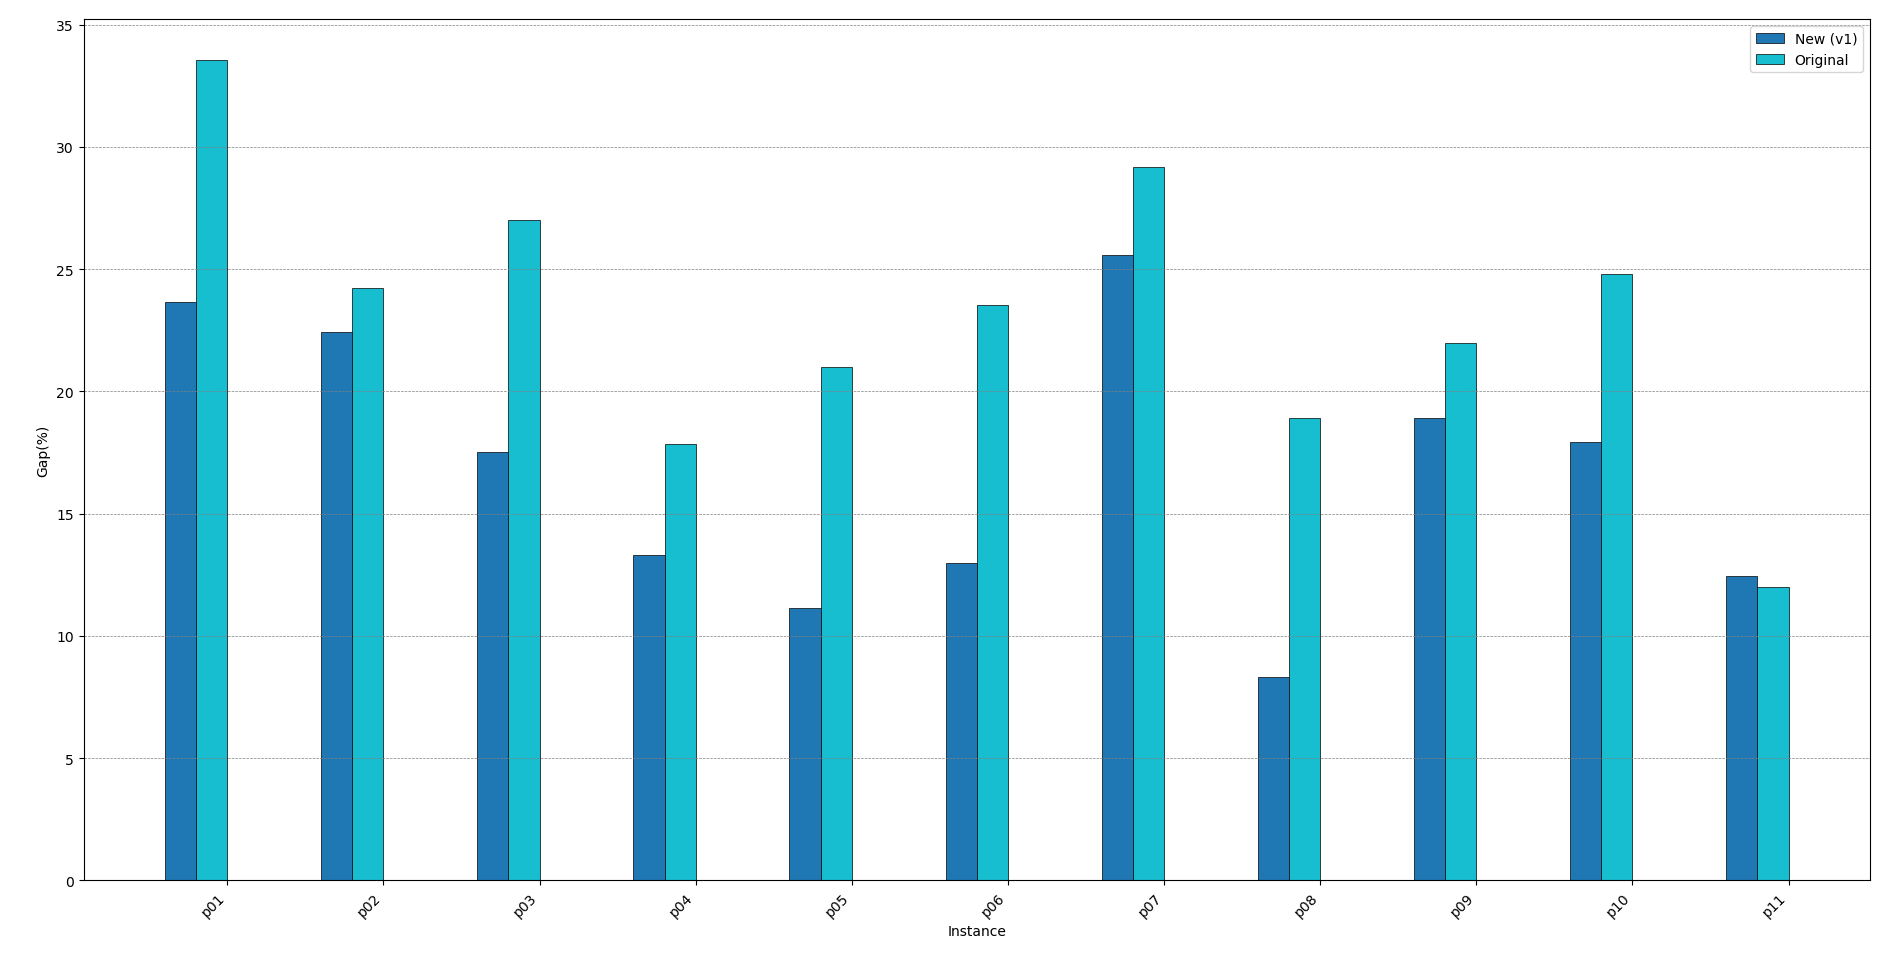
\includegraphics[width=\textwidth]{gaps_to_Hybrid_Standard}
		\centering
	\end{figure*}
	
	\begin{table}[h]
	\begin{minipage}{\columnwidth}
		\centering
		\caption{Performance Comparison (+Swap Local Optimization)}
		\resizebox{0.5\textwidth}{!}{%
			\begin{tabular}{@{}cccccc@{}}
				\toprule
				\textbf{Instance} & \textbf{Hybrid} & \textbf{New (v1)} & \textbf{gap(\%)} & \textbf{Original} & \textbf{gap(\%)} \\
				\midrule
				p01 & 180.03 & 217.42 & 20.77 & 243.72 & 35.38 \\
				\midrule
				p02 & 179.90 & 219.20 & 21.85 & 243.72 & 35.48 \\
				\midrule
				p03 & 174.47 & 214.84 & 23.14 & 277.50 & 59.05 \\
				\midrule
				p04 & 628.73 & 668.81 & 6.37 & 711.00 & 13.09 \\
				\midrule
				p05 & 583.01 & 630.78 & 8.19 & 713.00 & 22.30 \\
				\midrule
				p06 & 369.07 & 435.42 & 17.98 & 481.20 & 30.38 \\
				\midrule
				p07 & 271.82 & 309.48 & 13.85 & 322.29 & 18.57 \\
				\midrule
				p08 & 2809.48 & 3333.93 & 18.67 & 3448.84 & 22.76 \\
				\midrule
				p09 & 1753.60 & 1917.82 & 9.36 & 2201.39 & 25.54 \\
				\midrule
				p10 & 1259.76 & 1493.13 & 18.52 & 1630.94 & 29.46 \\
				\midrule
				p11 & 985.47 & 1145.75 & 16.26 & 1211.33 & 22.92 \\
				\midrule
				\textbf{Avg} & 835.94 & 962.42 & 15.91 & 1044.08 & 28.63 \\
				\bottomrule
			\end{tabular}%
		}
		\label{+Swap_comp_all_results}
	\end{minipage}
\end{table}\;
	\begin{figure*}[h]
		\caption[width=\textwidth]{Error percentage of the two versions to the best result found by H-AACONC (+Swap version of  Local Optimization)}
		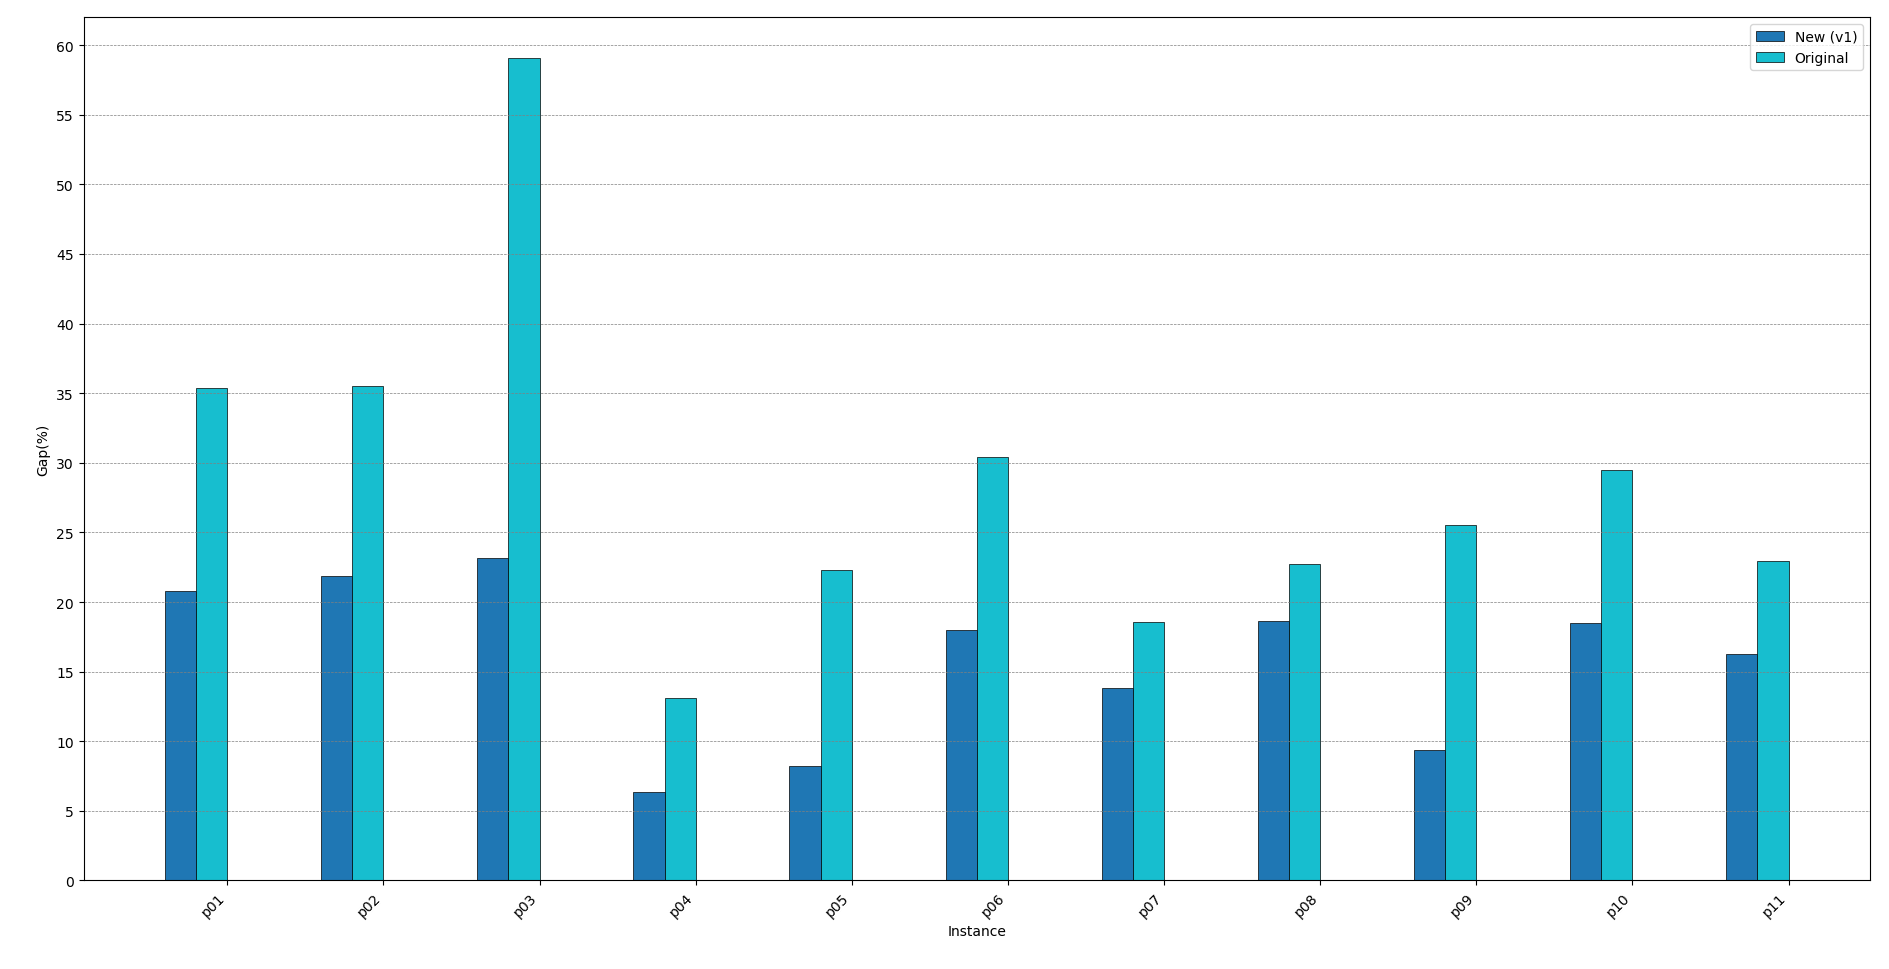
\includegraphics[width=\textwidth]{gaps_to_Hybrid_+Swap}
		\centering
	\end{figure*}
	\begin{figure*}[h]
		\caption[width=\textwidth]{Results (Standard Local Optimization)}
		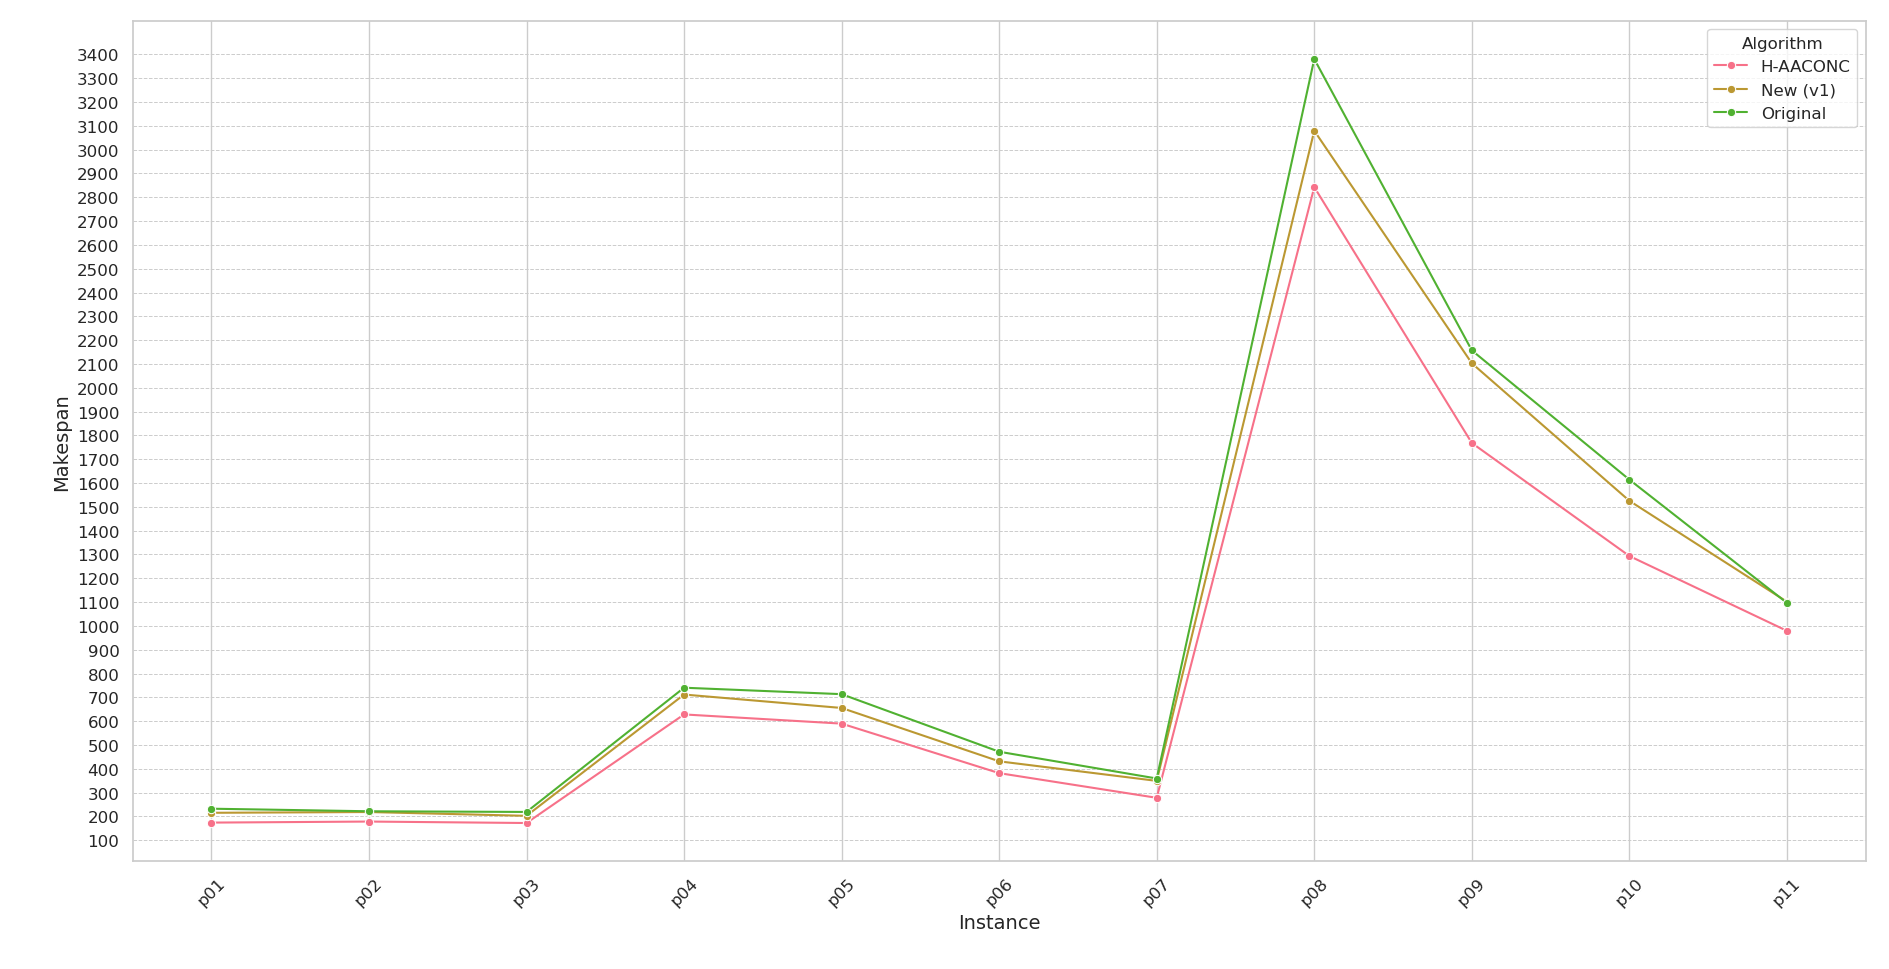
\includegraphics[width=\textwidth]{best_results_all_Standard}
		\centering
	\end{figure*}
	\begin{figure*}[h]
		\caption[width=\textwidth]{Results (+Swap Local Optimization)}
		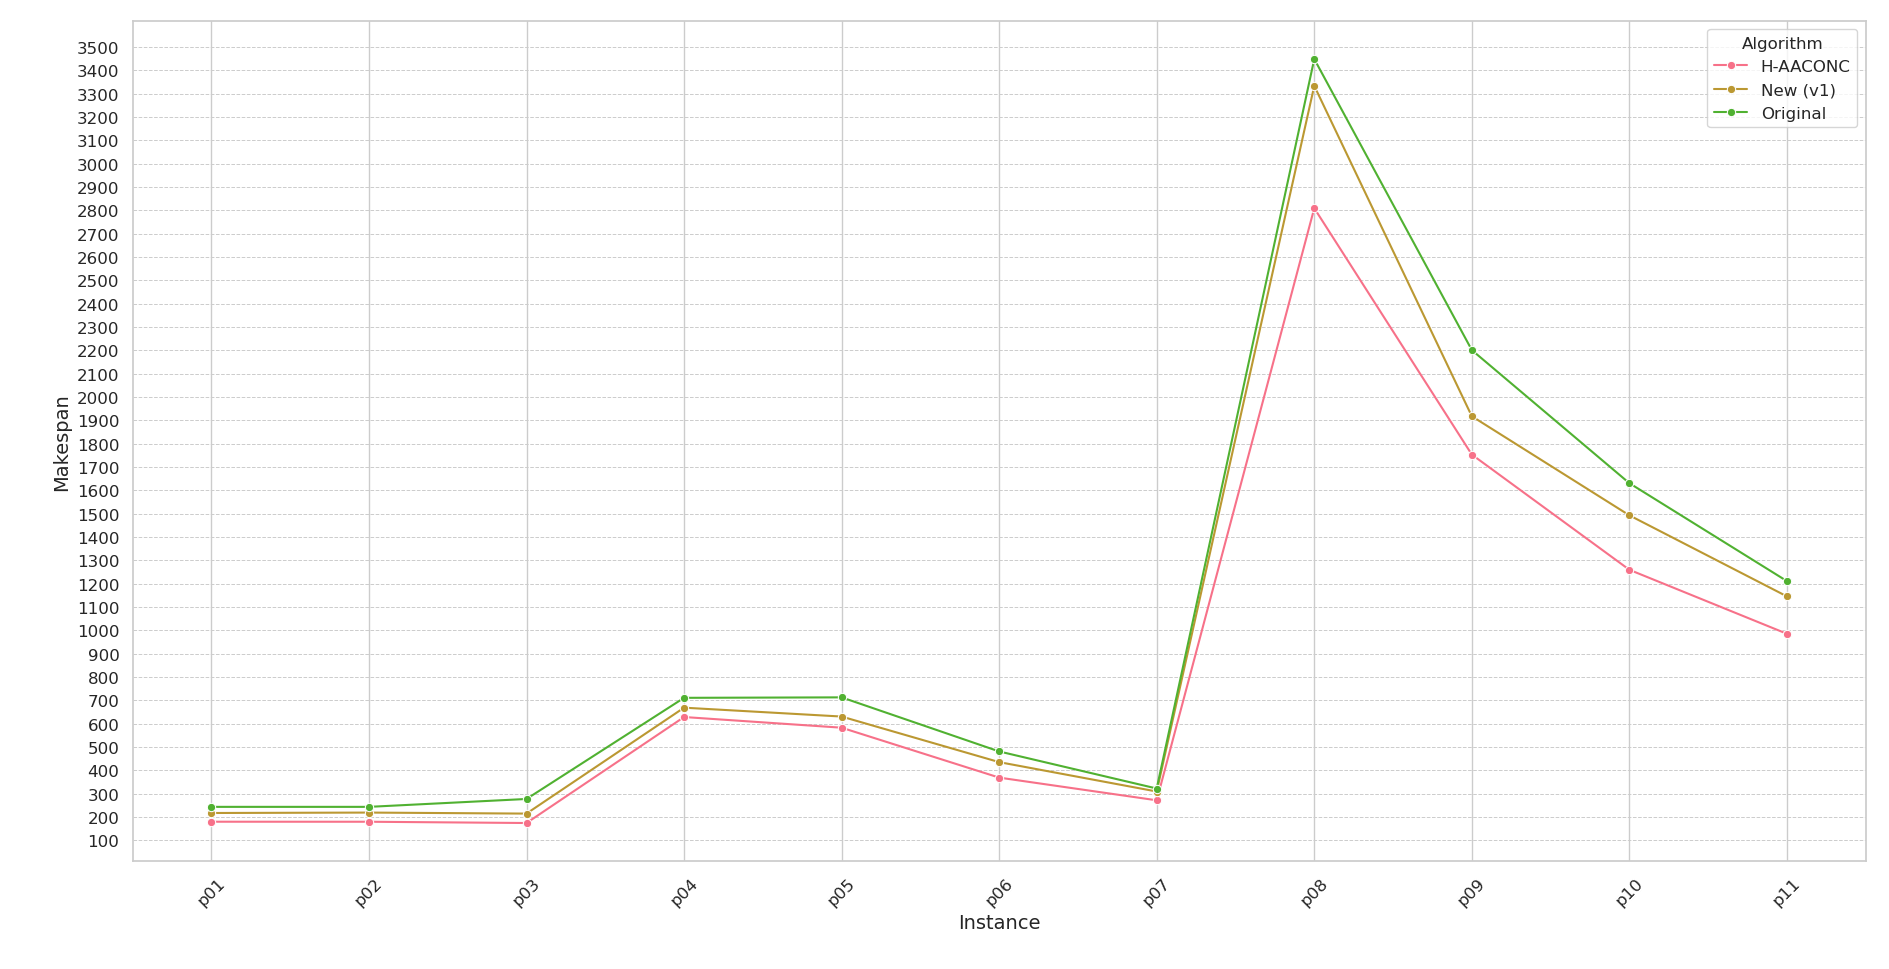
\includegraphics[width=\textwidth]{best_results_all_+Swap}
		\centering
	\end{figure*}
	
	
	\twocolumn
	
	\section{Related Literature}
	% Please add the following required packages to your document preamble:
% \usepackage{booktabs}
% \usepackage{graphicx}
\begin{table*}[]
	\caption{Drone-related Routing literature}
	\resizebox{\textwidth}{!}{%
		\begin{tabular}{@{}lllcccl@{}}
			\toprule
			\textbf{Reference} & \textbf{Problem} & \textbf{Scale} & \textbf{Tandem} & \textbf{Flight endurance} & \textbf{Capacitated*} & \textbf{Solution Method} \\ \midrule
			Murray \& Chu (2015) & FSTSP & 1-Truck 1-Drone 1-Depot & Yes & Yes & No & MILP, Heuristics \\
			\midrule
			& PDSTSP & 1-Truck n-Drone 1-Depot & No & Yes & No & MILP, Heuristics \\
			\midrule
			Ha et al. (2015) & FSTSP & 1-Truck 1-Drone 1-Depot & Yes & Yes & No & MIP, Heuristics \\
			\midrule
			Freitas \& Penna (2018) & FSTSP & 1-Truck 1-Drone 1-Depot & Yes & Yes & No & IP, Heuristics \\
			\midrule
			Boccia et al. (2021) & FSTSP/PDSTSP & 1-Truck 1-Drone 1-Depot & Yes & Yes & No & MILP, Heuristics \\
			\midrule
			Dell'Amico et al. (2021) & FSTSP & 1-Truck 1-Drone 1-Depot & Yes & Yes & No & MILP \\
			\midrule
			Dell'Amico et al. (2021) & FSTSP & 1-Truck 1-Drone 1-Depot & Yes & Yes & No & Branch and bound, Heuristic  \\
			\midrule
			Kuroswiski et al. (2023) & FSTSP & 1-Truck 1-Drone 1-Depot & Yes & Yes & No & MILP, Metaheuristics \\
			\midrule
			Pilcher (2023) & FSTSP & 1-Truck 1-Drone 1-Depot & Yes & Yes & No & Self-adaptive GA \\
			\midrule
			Mbiadou Saleu et al. (2018) & PDSTSP & 1-Truck n-Drone 1-Depot & No & Yes & No & MILP, Heuristics \\
			\midrule
			Dinh et al. (2021) & PDSTSP & 1-Truck n-Drone 1-Depot & No & Yes & No & Metaheuristics \\
			\midrule
			Nguyen et al. (2022) & PDSTSP & 1-Truck n-Drone 1-Depot & No & Yes & No & MILP \\
			\midrule
			Mbiadou Saleu et al. (2022) & PDSMTSP & m-Truck n-Drone 1-Depot & No & Yes & No & MILP, Metaheuristics \\
			\midrule
			Montemanni et al. (2023) & PDSTSP & 1-Truck n-Drone 1-Depot & Yes & Yes & No & Constraint Programming  \\
			\midrule
			Nguyen et al. (2023) & PDSTSP-c & 1-Truck n-Drone 1-Depot & No & Yes & No & MILP, Metaheuristics  \\
			\midrule
			Montemanni et al. (2024) & PDSTSP-c & 1-Truck n-Drone 1-Depot & No & Yes & No & MILP, Constraint Programming \\
			\midrule
			Ham (2018) & PDSTSP$^{+DP}$ & m-Truck n-Drone 2-Depot & No & Yes & No & Constraint Programming \\
			\midrule
			Agatz et al. (2018) & TSP-D & 1-Truck 1-Drone 1-Depot & Yes & Yes & No & IP, Heuristics \\
			\midrule
			Yurek et al. (2018) & TSP-D & 1-Truck 1-Drone 1-Depot & Yes & Yes & No & MIP, Heuristics \\
			\midrule
			Ha et al. (2018) & min-cost TSP-D & 1-Truck 1-Drone 1-Depot & Yes & Yes & No & MILP, GRASP, TSP-LS \\
			\midrule
			Dorling et al. (2016) & DDPs & 0-Truck n-Drone 1-Depot & No & Yes & Yes & MILP, SA \\
			\midrule
			Ulmer \& Thomas (2018) & SDDPHF & m-Truck n-Drone 1-Depot & No & No & No & Adaptive dynamic programming \\
			\midrule
			Salama \& Srinivas (2020) & JOCR & 1-Truck n-Drone 1-Depot & Yes & Yes & No & IP, MILP, Heuristics \\
			\midrule
			Lu et al. (2022) & FDTSP & 1-Truck n-Drone 1-Depot & Yes & Yes & No & Heuristics, Metaheuristics \\
			\midrule
			Lan (2024) & TSPTWD & 1-Truck 1-Drone 1-Depot & Yes & Yes & No & Metaheuristics \\
			\midrule
			Wang et al. (2017) & VRPD & m-Truck n-Drone 1-Depot & Yes & Yes & Yes & Problem formulation, theoretical study \\
			\midrule
			Schermer et al. (2018) & VRPD & m-Truck n-Drone 1-Depot & Yes & Yes & Yes & Heuristics \\
			\midrule
			Sacramento et al. (2019) & VRP-D & m-Truck m-Drone 1-Depot & Yes & Yes & Yes* & MIP, ALNS \\
			\midrule
			Schermer et al. (2019) & VRPDERO & m-Truck n-Drone 1-Depot & No & Yes & No & MILP, VNS, TS \\
			\midrule
			Nguyen et al. (2022) & PDSVRP & m-Truck n-Drone 1-Depot & No & Yes & Yes & MILP, Metaheuristics \\
			\midrule
			Schermer et al. (2019) & VRPD & m-Truck n-Drone 1-Depot & Yes & Yes & No & MILP, Matheuristic \\
			\midrule
			Wang \& Sheu (2019) & VRPD & m-Truck n-Drone 1-Depot & No & Yes & Yes & MIP, branch-and-price \\
			\midrule
			Euchi \& Sadok (2021) & VRP-D & m-Truck m-Drone 1-Depot & Yes & Yes & Yes & MILP, HGA \\
			\midrule
			Lei et al. (2022) & VRPD & m-Truck m-Drone 1-Depot & Yes & Yes & Yes & Dynamical Artificial Bee Colony \\
			\midrule
			Karak et al. (2019) & HVDRP & m-Truck n-Drone 1-Depot & Yes & Yes & Yes(Drones) & MIP, Heuristics \\
			\midrule
			Kuo et al. (2022) & VRPDTW & m-Truck m-Drone 1-Depot & Yes & Yes & Yes & MIP, VNS \\
			\midrule
			Stodola et al. (2024) & MDVRP-D & m-Truck m-Drone m-Depot & Yes & Yes & Yes & ACO \\
			\midrule
			Oikonomou et al. (2019) & mfcmTSP & 1-Truck 1-Drone 1-Depot & No & No & No & Heuristics \\
			\midrule
			This paper & MD-mfcmTSP & m-Truck n-Drone k-Depot & No & No & Yes & Metaheuristics, Heuristics \\
			\bottomrule
		\end{tabular}%
	}
\end{table*}
	At the same time, it is important that we address flight range limitations. Such limitations have important roles in much of
	the existing drone routing research. However, even he first drones developed by Amazon and JD.com ahad a flight range of 15
	to 20 miles [33, 56]. Such a range is suitable to allow out and back travel in the medium-sized cities in which the authors live,
	Braunschweig, Germany, and Iowa City, United States. In fact, it is suitable for many larger cities such as Hamburg, Munich,
	and Paris. Thus, in contrast to other drone applications, in this work, we do not consider flight range as a limiting factor (Ulmer \& Thomas (2018)).
	
	\clearpage
	\section{Initial approach to AACONC+}
	\begin{algorithm}
		\caption{AACONC+ Algorithm}
		\SetAlgoNlRelativeSize{-1}
		
		\SetKwProg{Fn}{Function}{}{}
		
		\Fn{AACONC+($V, n_{\text{ants}}, n_{\text{freq}}, n_{\text{size}}, n_{\text{sect}}, n_{\text{prim}}, T_{\text{update}}, \alpha, \beta, \rho_{\text{min}}, \rho_{\text{max}}, \delta$)}{
			$|R| = \infty$\;
			$iter = 0$\;
			Initialize pheromone matrices $\tau$\;
			
			\For{each $v_i \in V$}{
				$K(v_i)=$ CreateClusters($V, v_i, n_{\text{size}}, n_{\text{sect}}$)\;
			}
			
			\While{not terminated}{
				$|R_{\text{best}}| = \infty$\;
				$iter = iter + 1$\;
				
				\For{$a = 1$ to $n_{\text{ants}}$}{
					$R_a =$ AntSolution($V, K, \tau, \alpha, \beta$)\;
					
					\If{$|R_a| < |R_{\text{best}}|$}{
						$R_{\text{best}} = R_a$\;
					}
				}
				\If{$iter \mod n_{\text{freq}} = 0$}{
					$R_{\text{best}} =$ LocalOptimization($V, R_{\text{best}}$)\;
				}
				\If{$|R_{\text{best}}| < |R|$}{
					$R = R_{\text{best}}$\;
				}
				Update pheromone matrices $\tau$\;
				Calculate evaporation coefficient $\rho$\;
				Evaporate pheromone matrices $\tau$ using $\rho$\;
			}
			
			\textbf{return} $R$\;
		}
\end{algorithm}
\;
		
	\begin{algorithm}
		\caption{antSolution}
		
		\SetKwProg{Fn}{Function}{}{}
		
		\Fn{antSolution($V = \{D,C\}, K, \tau, \alpha, \beta$)}{
			$V_{free}$ = $C$\;
			
			\While{$V_{\text{free}} \neq \emptyset$}{
				$vt = $ selectVehicleType($V_{free}, K, \tau$)\\
				$d = $ selectDepot($vt, V_{free}, K^{(vt)}, \tau$)\\
				$v = $ selectVehicle($vt, d, V_{free}, K^{(vt)}, \tau$)\\
				
				$pos \leftarrow$ \text{vehicle's position}\
				
				$k = $ selectCluster($vt, d, v, V_{free}, K^{(pos)(vt)}, \tau, \alpha, \beta$)\
				
				$V_{candidates} = V_{\text{free}} \cap K_k^{(pos)(vt)}$\
				
				
				$c = $ selectCustomer($vt, d, pos, V_{candidates}, \tau, \alpha, \beta$)\\
				\uIf(//Drone serves customer and immediately returns to depot){vt = Drone}{
					$R_d^{vt} = R_d^{vt} + \{c\}$\\
					$R_d^{(vt)} = R_d^{(vt)} + \{d\}$\\
				}
				\Else{	
					\If{$v_{load} < c^{(demand)}$}{
						$R_d^{(vt)} = R_d^{(vt)} + \{d\}$\\
						$v_{load} = vt_{capacity}$\\
					}
					$R_d^{vt} = R_d^{vt} + \{c\}$\\
					$v_{pos} = \{c\}$\\
					$v_{load} = v_{load} - {c^{(demand)}}$\\
				}
				$V_{\text{free}} = V_{\text{free}} - \{c\}$\\
			}
			\ForEach(//Vehicles return to their depots){$d \in D \text{ and } vt\in VT$}{$R_d^{vt} = R_d^{vt} + \{d\}$}\
			\textbf{return} $R = \{R_1^1, R_2^1, ..., R_2^3, R_3^3, ...,R_D^{VT}\}$\
		}
		\end{algorithm}
\;
	
	
	\begin{algorithm}
		\caption{selectVehicle}
		\SetKwProg{Fn}{Function}{}{}
		
		\Fn{selectVehicle($vt, d, V_{free}, K^{(vt)}, \tau$)}{
				\For{each $v_i\in Vh^{(vt)(d)}$}{
					$V_{\text{cand}} = \emptyset$\\
					$pos \leftarrow$\text{vehicle's current location}\
					
					\For{\text{k = 1 to} $n_{prim}$}{
						$V_{cand} = V_{cand} + V_{free} \cap K_k^{(vt)(pos)}$\
					}
					
					$p(v_i) = \sum_{v_j \in V_{cand}} \tau_{v_{pos} v_j}^{(vt)(d)}$\
				}
			$p_{sum} = \sum_{v_i \in V^{(vt)(d)}} p(v_i)$\\
			$p(v_i) = p(v_i)\div p_{sum}$\\
			Select $v_i\in Vh^{(vt)(d)}$ based on probabilities $p(v_i)$ using roulette wheel\\
			\textbf{return} $v_i$\;
		}
		
	\end{algorithm}

\;
	\newpage
	\subsection{AACONC+ Results and Comparison to heuristics}
	% Please add the following required packages to your document preamble:
% \usepackage{booktabs}
% \usepackage{graphicx}
\begin{table*}[!ht]
	\begin{minipage}{\columnwidth}
		\centering
		\caption{AACONC+ Results}
	\resizebox{\textwidth}{!}{%
		\begin{tabular}{@{}ccccccc@{}}
			\toprule
			\textbf{Instance} & \textbf{Best} & \textbf{Average} & \textbf{gap(\%)} & \textbf{Worst} & \textbf{gap(\%)} & \textbf{Average time(s)} \\
			\midrule
			p01-C & 178.56 & 196.74 & 10.18 & 225.60 & 26.34 & 141 \\
			\midrule
			p02-C & 172.73 & 196.57 & 13.8 & 234.78 & 35.92 & 123 \\
			\midrule
			p03-C & 173.82 & 187.26 & 7.73 & 210.15 & 20.90 & 305 \\
			\midrule
			p04-C & 629.88 & 644.84 & 2.37 & 675.63 & 7.26 & 1203 \\
			\midrule
			p05-C & 573.03 & 613.47 & 7.06 & 692.44 & 20.84 & 884 \\
			\midrule
			p06-C & 379.10 & 390.34 & 2.96 & 403.39 & 6.41 & 1316 \\
			\midrule
			p07-C & 288.24 & 297.91 & 3.35 & 314.78 & 9.21 & 798 \\
			\midrule
			p08-C & 3023.77 & 3100.23 & 2.53 & 3265.97 & 8.01 & 1635 \\
			\midrule
			p09-C & 1705.03 & 1774.86 & 4.10 & 1846.92 & 8.32 & 3391 \\
			\midrule
			p10-C & 1286.28 & 1319.78 & 2.60 & 1349.47 & 4.91 & 3549 \\
			\midrule
			p11-C & 992.16 & 1035.63 & 4.38 & 1061.7 & 7.01 & 3600 \\
			\midrule
			p12-C & 1082.12 & 1123.30 & 3.81 & 1175.39 & 8.62 & 446 \\
			\midrule
			p13-C & 1099.02 & 1135.30 & 3.30 & 1191.96 & 8.46 & 491 \\
			\midrule
			p14-C & 1111.12 & 1123.33 & 1.10 & 1170.17 & 5.31 & 423 \\
			\midrule
			p15-C & 1166.08 & 1202.57 & 3.13 & 1228.27 & 5.33 & 2471 \\
			\midrule
			p16-C & 1178.51 & 1209.60 & 2.64 & 1241.67 & 5.36 & 2146 \\
			\midrule
			p17-C & 1142.74 & 1199.88 & 5.00 & 1253.47 & 9.69 & 2628 \\
			\midrule
			p18-C & 1231.96 & 1263.90 & 2.59 & 1296.42 & 5.23 & 3368 \\
			\midrule
			p19-C & 1250.26 & 1266.54 & 1.30 & 1284.23 & 2.72 & 3600 \\
			\midrule
			p20-C & 1246.36 & 1266.70 & 1.63 & 1280.77 & 2.76 & 3445 \\
			\midrule
			p21-C & 1296.19 & 1330.11 & 2.62 & 1347.09 & 3.93 & 3600 \\
			\midrule
			p22-C & 1317.94 & 1332.07 & 1.07 & 1354.61 & 2.78 & 3600 \\
			\midrule
			p23-C & 1319.93 & 1341.50 & 1.63 & 1356.62 & 2.78 & 3600 \\
			\midrule
			\textbf{Average} & 1037.52 & 1067.59 & 3.46 & 1107.25 & 8.68 & 2021.13 \\ \bottomrule
		\end{tabular}%
	}
	\label{tab:table2}
\end{minipage}
\end{table*}\;
	% Please add the following required packages to your document preamble:
% \usepackage{booktabs}
% \usepackage{graphicx}
% \usepackage{amsmath}
\begin{table*}[h!]
	\begin{minipage}{0.7\columnwidth}
		\centering
		\caption{AACONC+ best and heuristic results}
		\resizebox{\textwidth}{!}{%
			\begin{tabular}{@{}cccccc@{}}
				\toprule
				\textbf{Instance} & \textbf{AACONC+} & \textbf{heuristic (prox.)} & \textbf{gap(\%)} & \textbf{heuristic (k-means)} & \textbf{gap(\%)} \\
				\midrule
				p01-C & \textbf{178.56} & 217.42 & 21.76 & 191.03 & 6.98 \\
				\midrule
				p02-C & \textbf{172.73} & 219.2 & 26.90 & 188.60 & 9.19 \\
				\midrule
				p03-C & \textbf{173.82} & 214.84 & 23.60 & 185.82 & 6.90 \\
				\midrule
				p04-C & \textbf{629.88} & 668.81 & 6.18 & 694.96 & 10.33  \\
				\midrule
				p05-C & \textbf{573.03} & 630.78 & 10.08 & 624.33 & 8.95  \\
				\midrule
				p06-C & \textbf{379.10} & 435.42 & 14.86 & 416.25 & 9.80 \\
				\midrule
				p07-C & \textbf{288.24} & 309.48 & 7.37 & 314.41 & 9.08 \\
				\midrule
				p08-C & \textbf{3023.77} & 3333.93 & 10.26 & 3186.02 & 5.37  \\
				\midrule
				p09-C & \textbf{1705.03} & 1917.82 & 12.48 & 1964.49 & 15.22 \\
				\midrule
				p10-C & \textbf{1286.28} & 1493.13 & 16.08 & 1500.38 & 16.64  \\
				\midrule
				p11-C & \textbf{992.16} & 1145.75 & 15.48 & 1031.09 & 3.92  \\
				\midrule
				p12-C & \textbf{1082.12} & 1273.77 & 17.71 & 1273.77 & 17.71 \\
				\midrule
				p13-C & \textbf{1099.02} & 1226.63 & 11.61 & 1226.63 & 11.61  \\
				\midrule
				p14-C & \textbf{1111.12} & 1284.73 & 15.62 & 1284.73 & 15.62  \\
				\midrule
				p15-C & \textbf{1166.08} & 1347.67 & 15.57 & 1295.23 & 11.08 \\
				\midrule
				p16-C & \textbf{1178.51} & 1289.29 & 9.40 & 1289.29 & 9.40 \\
				\midrule
				p17-C & \textbf{1142.74} & 1320.91 & 15.59 & 1273.39 & 11.43  \\
				\midrule
				p18-C & 1231.96 & 1260.24 & 2.30 & \textbf{1211.56} & -1.66  \\
				\midrule
				p19-C & 1250.26 & 1266.92 & 1.33 & \textbf{1248.93} & -0.11  \\
				\midrule
				p20-C & 1246.36 & 1323.10 & 6.16 & \textbf{1234.12} & -0.98  \\
				\midrule
				p21-C & 1296.19 & 1363.18 & 5.17 & \textbf{1231.23} & -5.01  \\
				\midrule
				p22-C & 1317.94 & 1295.67 & -1.69 & \textbf{1230.99} & -6.60  \\
				\midrule
				p23-C & 1319.93 & 1252.36 & -5.12 & \textbf{1222.63} & -7.37 \\
				\midrule
				\textbf{Average} & \textbf{1037.52} & 1134.39 & 11.24 & 1100.86 & 6.84 \\ \bottomrule
			\end{tabular}%
		}
	\end{minipage}
\end{table*}
\;
	\captionsetup{justification=centering}  % Center the captions


	
\end{document}